\documentclass[12pt,letterpaper ,oneside , openright]{book}
\usepackage{thesis}
%para desarrollo
	%\usepackage{showframe}
	%\includeonly{calculatingProperties_chapter,calculatingProperties/parameters,calculatingProperties/enthalpy}
%--

\begin{document}
	\begin{titlepage}
	\begin{minipage}[c][9in][s]{1in}
	\centering
	
\includegraphics[width=1in]{Escudo-UNAM}\\[10pt]
	\hskip 2pt\vrule width 2pt height 6.7in
	\hskip 1mm\vrule width 1pt height 6.7in\\[10pt]
	
\includegraphics[width=1in]{images/FQ.jpg}
	\end{minipage}\hskip 10pt
	\begin{minipage}[c][\textheight][s]{5.125in}
	\centering
	{\textsc{ \large{Universidad Nacional Autónoma De México}}}
	\vspace{3mm}\hrule height2pt
	\vspace{1mm}\hrule height1pt
	\vspace{3mm}
	\textsc{Facultad De Química}\\[3cm]
	\textsc{\Large Desarrollo de una librería en java para el cálculo de propiedades de sustancias con ecuaciones de estado cúbicas}\\[3cm]
	\makebox[8cm][s]{\Huge T E S I S}\\[8pt]
	\textsc{ que para obtener el título de }\\[3pt]
	\textsc{ Ingeniero Químico}\\[1cm]
	\textsc{ presenta: }\\[0.3cm]
	\textsc{ Hugo Redon Rivera }\\[0.5cm]
	\vfill
	{\scshape {México, D.F.} \hfill{2014} }	
	\end{minipage}
\end{titlepage}
\newpage
\begin{minipage}[c][\textheight][s]{5.125in}
JURADO ASIGNADO:\\[0.5cm]

PRESIDENTE:		Profesor:\\
VOCAL: 		Profesor:\\
SECRETARIO:		Profesor:\\
1er.  SUPLENTE: 	Profesor:\\
2° SUPLENTE:		Profesor:\\[0.5cm]

\begin{center}
	SITIO DONDE SE DESARROLLÓ EL TEMA:\\
	\textsc{Facultad de Química}\\[3cm]


	\rule{6cm}{1pt}\\
	\textsc{asesor del tema: Dr. Enrique Rodolfo Bazúa Rueda.} \\[3cm]


	\rule{6cm}{1pt}\\
	\textsc{SUSTENTANTE:Hugo Redon Rivera.} 
\end{center}
\end{minipage}
%Portada -Hecho
	\tableofcontents	
	\chapter{Objetivos}

\begin{itemize}
	\item Desarrollar una biblioteca escrita en el lenguaje de java para realizar:
	\begin{itemize}
		\item El cálculo de propiedades de sustancias puras y mezclas con ecuaciones de estado cúbicas.
		\item Cálculos de equilibrio Líquido-Vapor.
		\item La estimación de parámetros de expresiones de $\alpha$ para el cálculo de la constante $a$ de la ecuación de estado cúbica.
		\item La estimación de parámetros binarios de las reglas de mezclado para el cálculo de las constantes $a$ y $b$ para mezclas.
	\end{itemize}
	\item La biblioteca a desarrollar deberá ser versátil, robusta, simple de usar y fácilmente expandible.
	\item Desarrollar una interfaz de usuario que exponga las funciones de la librería.
	\item Proponer un medio de difusión de la librería, que sea capaz de involucrar a cualquier persona interesada en modificar y extender la librería.
\end{itemize}

\chapter{Introducción}

	Esta tesis trata sobre el uso de métodos computacionales para el cálculo de propiedades volumétricas y puntos de equilibrio Líquido-Vapor con ecuaciones de estado cúbicas. 

	Como resultado se ha escrito una biblioteca de clases en java denominada \textbf{Materia}.

	El diseño de la biblioteca en conjunto con las herramientas que se describen en la sección \ref{chap:tools} hacen de este trabajo una plataforma para el desarrollo de aplicaciones de simulación y modelado de procesos quimicos industriales.

	El presente trabajo propone un procedimiento para el desarrollo de futuras aplicaciones. Para lo cual se ha dotado de ciertas características a la biblioteca \textbf{Materia} asegurando el funcionamiento del proceso propuesto.

	La biblioteca \textbf{Materia} se ha escrito para que su utilizacióń sea sencilla y no se requieran grandes conocimientos sobre programación. El capítulo \ref{chap:libraryUse} muestra como utilizar la estructura de clases para realizar los cálculos de propiedades y de equilibrio, mostrando pequeños fragmentos de código.

	El capítulo \ref{chap:libraryExtension} muestra como extender la biblioteca de clases, guía en el proceso de creación de nuevas reglas de mezclado, expresiones de $\alpha$, etc. Este capítulo supone un conocimiento mas avanzado en temas de programación orientada a objetos.

	Se ha creado una página de internet para permitir el uso de la librería \textbf{Materia} a través de una interfaz de usuario, el capítulo \ref{chap:webPage} documenta las funciones de la página. También es posible extender las funciones de la página de internet, sin embargo son necesarios conocimientos que estan fuera del alcance de esta tesis. El apéndice \ref{chap:webTools} describe las tecnologías utilizadas para la creación de la página de internet, y una breve descripción de su estructura.
	%\marginpar{Explicación de las ecuaciones y cálculos que se realizan,Versatilidad del programa,Descripción de la estructura de la tesis,Alcance de la aplicación}
	%Objetivos -Hecho
	\chapter{Herramientas}
	\section{Java}
		Un lenguaje simple, orientado a objetos, distribuido, interpretado, robusto, de arquitectura neutral, portátil, de alto rendimiento, seguro, multiproceso y dinámico.\cite{java} 

		Definición dada por James Gosling \footnote{Considerado creador del lenguaje Java}  en la fecha de su primer publicación (1995). 

		\begin{description}
		\item{Simple:} Una de las razones mas importantes por las que se decidió programar la librería en este lenguaje es que java evita al programador la necesidad de realizar tareas de índole técnico sobre la computadora, como por ejemplo el almacenamiento de los datos en la memoria. Esto permite al programador concentrarse en el area de estudio deseada.

		\item{Orientado a objetos:}
		Sin duda la perspectiva orientada a objetos de java es otro gran atractivo para las ciencias e ingenierías. La división y clasificación de las ramas de estudio permiten concentrarnos en todos y cada uno de los aspectos importantes sobre el tema. De igual manera la division de un programa en objetos nos permite concentrarnos en los aspectos y actividades importantes. Tómese como ejemplo la clasificación de la materia en homogénea y heterogénea, el aspecto importante en esta clasificación es la presencia de uno o más estados de agregación en el sistema, se puede pensar así en un cálculo de equilibrio Líquido-Vapor para un sistema heterogéneo, pero no para un sistema homogéneo.

		\item{Distribuido:}
		Java es una de las principales herramientas para el desarrollo web, un invento solo comparable con la imprenta. Su importancia radica en su capacidad de difusión masiva. La creación de un servicio o cualquier producto es tan importante como su difusión. En conjunto con la librería de funciones se ha creado un sitio web donde se exponen algunas de las funciones mas importantes de la librería.

		\item{De arquitectura neutra:}
		Java es multiplataforma, lo cual significa que puede ser ejecutado en la gran mayoría de los sistemas operativos existentes en el mercado actual.

		\end{description}

	\section{JUnit}

		Esta librería de funciones \footnote{Librería de funciones es una traducción de ``java class library'', que es el nombre del tipo de proyecto del presente trabajo. Una mejor definicion sería una ``Estructura de objetos''} ha sido creada con la idea de expandirse y ser escrita por cualquier persona interesada en ello.Es muy importante mantener una evidencia del funcionamiento de la librería. El uso de la tecnología JUnit es una forma para asegurar que los cambios introducidos al programa no han afectado el funcionamiento esperado de la libreria.

		Al momento de escribir este trabajo la librería cuenta con mas de 100 pruebas que definen un funcionamiento.

		\subsection{Desarrollo basado en pruebas}
	\section{Git}

		Git es un sistema de gestión y distribución de código fuente. Permite llevar un registro de los cambios realizados, utilizar las diferentes versiones, y compartir los cambios entre usuarios.

	\section{GitHub}

		GitHub es un servicio de depósitos de repositorios Git. Es un sitio donde se puede guardar el código fuente, es muy fácil contribuir al proyecto y compartir los cambios propuestos, es accesible a todo el público.

	\section{Maven}

		Maven es una herramienta de construcción de código, una de sus grandes ventajas es que puede descargar de manera segura versiones compiladas de proyectos con unas pocas lineas de código. Mas adelante se detallara el proceso de uso.

	\section{Netbeans}
		NetBeans es un entorno de desarrollo integrado para el desarrollo principalmente con Java, pero también con otros lenguajes, en particular, PHP, C / C++, y HTML5. También es una estructura la plataforma de aplicaciones para aplicaciones de escritorio Java y otros.
	

	\section{Openshift}
		OpenShift es una plataforma de programación en la nube orientada a servicios de Red Hat. Una versión para la nube privada se llama OpenShift Enterprise. El software que ejecuta el servicio se encuentra bajo el nombre "OpenShift Origin" de código abierto y está disponible en GitHub.

	\section{Wildfly}
		WildFly, anteriormente conocido como "JavaBeans Open Source Software Application Server" es un servidor de aplicaciones que implementa la plataforma Java, Enterprise Edition. JBoss está escrito en Java y como tal es multiplataforma: utilizable en cualquier sistema operativo que soporte Java

	\section{GNU GENERAL PUBLIC LICENSE Version 2}

		"GNU GENERAL PUBLIC LICENSE" es una licencia libre, sin derechos para software y otro tipo de obras. Pretende garantizar la libertad de compartir y modificar todas las versiones de un programa - para asegurarse de que sigue siendo software libre para todos sus usuarios.
		
	\section{Idioma}

		Existen dos razones por la que se ha elegido el idioma inglés para expresar las funciones de la librería. La primer razon y las mas importante, es que java ha sido escrito en inglés y por lo tanto las estructuras de control y palabras reservadas. Pongamos como ejemplo el siguiente fragmento de código.

\begin{lstlisting}
public boolean isItADog(Pet pet){
	if ( pet.getSpeciesName().equals("Canis lupus familiaris")) {
		return true;
	}else{
		return false;
	}
}
\end{lstlisting}

	El fragmento de código pretende conocer si el nombre de la especie de la mascota es el nombre científico "Canis lupus familiaris", si es asi devuelve verdadero, de lo contrario falso. Veamos ahora la versión en español para el mismo fragmento de código.

\begin{lstlisting}
public boolean esUnPerro(Mascota mascota){
	if ( mascota.getNombreDeLaEspecie().equals("Canis lupus familiaris")){
		return true;
	}else{
		return false;
	}
}
\end{lstlisting}

	En inglés, el order de las palabras denota la diferencia entre una pregunta y una afirmación, de modo que el nombre del método en inglés claramete indica la pregunta "Is it a Dog?" cuando en español la diferencia entre la pregunta y la afirmación debe ser escrita con un signo de interrogación "¿Es un perro?" sin ellos el nombre del metodo puede parecer la afirmación "Es un perro!".

	También puede notarse el nombre del método "getNombreDeLaEspecie", el prefijo "get" es una convención en java que significa recuperar, se usa para obtener el valor de la variable que continúe al prefijo, sin el prefijo estaríamos restringiendo la funcionalidad de la librería.

	Puede apreciarse que la lectura de la línea en ingles es fluida.No existe la necesidad de realizar traducciones. Aunque parezca trivial en este ejemplo, en porciones mas grandes de código la diferencia es bastante notable.

	Quiero hacer notar que en ningún momento se intenta hacer una comparación sobre los idiomas, sino señalar el beneficio de la fluidez que se obtiene al no mezclarlos.

	%Sobre java y herramientas -Hecho
	\chapter{Instalación}

  Para instalar la biblioteca \textbf{Materia} es necesario saber que tipo de trabajo se desea realizar con ella:
  \begin{itemize}
    \item Crear una aplicación que emplea las funciones ya definidas en la biblioteca.
    \item Crear una nueva funcionalidad de la biblioteca.
  \end{itemize}

  Por ejemplo si se desea escribir una aplicación que realize diagramas de presión contra volumen molar usando ecuaciones de estado cúbicas, solo será necesario instalar la forma compilada según la sección \ref{sec:compiledinstall}. Ya que las funciones para calcular la presión y el volumen molar con ecuaciones de estado cúbicas existen en la biblioteca , no será necesario modificar el código fuente, por lo tanto no es necesaria la instalación del código fuente. En cambio si se desea utilizar ecuaciones viriales para realizar los diagramas de presión, se deberán realizar las dos instalaciones descritas en este capítulo, ya que las ecuaciones viriales no forman parte del alance de esta tesis, la librería debera ser extendida para incluir dichas ecuaciones, una vez hecha la extensión al código fuente , la versión compilada puede ser empleada para realizar la aplicación que realice los diagramas.


  \section{Para uso de la librería (compilado)}\label{sec:compiledinstall}

      Existen dos formas de utilizar la librería Materia en una aplicación java:
    Descargar el archivo .jar y agregarlo al folder /lib de la aplicación ó desde maven utilizando el archivo pom.xml.

    La librería existe como un archivo .jar, se puede descargar desde la página creada para su difusión \url{ingenieria-eqpro.rhcloud.com}, o automáticamente desde los servidores de sonatype haciendo uso de maven.

    Si se realiza la instalación manual la ubicación de la librería depende de la estructura del proyecto, por ejemplo para una aplicación web los archivos jar deberán ser agregados en el folder dentro del proyecto src/main/webapp/WEB-INF/lib.

    Utilizando maven solo deberán agregarse las siguientes lineas de código al archivo pom.xml.

    \begin{lstlisting}[language=XML,morekeywords={repositories,
    repository,id,name,url,groupId,artifactId,dependencies,dependency}]
<dependencies>
  <dependency>
   <groupId>com.github.hugoredon</groupId>
   <artifactId>materia</artifactId>
   <version>1</version>
  </dependency>
</dependencies>
\end{lstlisting}

    En el apéndice \ref{sec:manualInstall} se ejemplifica la instalación manual y en el apéndice \ref{sec:mavenInstall} se muestra la instalación vía maven, para una aplicación de escritorio.


  \section{Para extender o modificar la librería (código fuente)}

    El código fuente de la librería se expone de manera pública en la página \url{https://github.com/HugoRedon/Materia}, bajo la licencia GNU GENERAL PUBLIC LICENSE Version 2.
  
    Para poder participar en el proyecto será necesario obtener de manera gratuita una cuenta en github, realizar una copia o clon \footnote{En github a una copia de un proyecto se conoce como ``Fork''} de la librería  a la nueva cuenta, copiar el código fuente a la computadora haciendo uso de git,realizar los cambios y agregarlos a la cuenta en GitHub  \footnote{El procedimiento hace uso de los comandos `git clone', `git commit' y `git push', que son explicados con mas detalle en el apéndice \ref{chapgithub}} ,finalmente hacer una petición para integrar los cambios a la librería original ``Pull request'', y si los cambios son aceptados, se habrá logrado la participación al proyecto. El proceso se detalla en el apéndice \ref{chap:github}.



%Sobre la instalación Hecho
	\chapter{Cálculos}
	



	\section{Propiedades}	
		\section{Ecuación de estado cúbica}
 La presión es el cálculo mas sencillo que podemos realizar con la ecuación de estado cúbica.

\begin{equation}
	p = \frac{R T}{v-b} - \frac{a}{v^2 +u b v + w b^2 }
\end{equation}

 Crearemos una clase en java que use la librería Materia y realize una gráfica de presión contra volumen a una temperatura determinada.

%\pgfplotstabletypeset{plotdata/pressurevolume.dat}%no es necesario mostrar la tabla

\begin{tikzpicture}
\begin{axis}
\addplot[blue]table{plotdata/pressurevolume.dat};
\end{axis}
\end{tikzpicture}


\begin{tikzpicture}
\begin{axis}
\addplot3[surf,
colormap={blueblack}{color=(white) color=(blue)},
domain=0:1]table{plotdata/pressurevolumetemperature.dat};
\end{axis}
\end{tikzpicture}


\begin{lstlisting}[label=se,caption=Some Code]
Cubic cubic = new Cubic();
//parametros de van der waals para el heptano
double a = 3107000.0;
double b = 0.2049;


double min_volume = 0.245;
double max_volume = 2.06;

int n = 100;
double pass = (max_volume- min_volume)/n;

PrintWriter writer = new PrintWriter(fileName, "UTF-8");
writer.println(" Volumen Presion");
for(int i=0;i < n; i++){
	double volume = min_volume + pass*i;
	double pressure = cubic.calculatePressure(300, volume, a, b);
	
	writer.println(" "+ volume + " " + pressure);
}
writer.close();		
\end{lstlisting}



















		


		\subsection{Entalpía}

\begin{equation}
h = h^{\neq} + \left[ \frac{T(\frac{\partial a}{\partial T}) - a}{b\sqrt{u²-4w} }\right] 
\ln\left[\frac{2v+b\left(u + \sqrt{u²-4w}\right)}{2v+b\left(u - \sqrt{u²-4w}\right)}\right]
+ pv - RT
\end{equation}

\begin{lstlisting}[label=some-code,caption=Some Code]
private  double calculateEnthalpy( double volume){
    double idealGasEnthalpy = calculateIdealGasEnthalpy();
    double a = calculate_a_cubicParameter();
    double b = calculate_b_cubicParameter();
    double L = cubicEquationOfState.calculateL(volume, b);
    double partial_aPartial_temperature = partial_aPartial_temperature( );
    
    return idealGasEnthalpy + ((partial_aPartial_temperature - a)/b) * L  + pressure * volume - Constants.R *temperature;
}
\end{lstlisting}	


\subsubsection{Entalpía del gas ideal}
\begin{equation}
h^{\neq} = \sum_{i=1}^{nc} x_i \left[ h_i^{ref} + \int_{Tref}^{T} Cp_i^{\neq} \mathrm{d}T \right]
\end{equation}



\begin{tikzpicture}
\begin{axis}
\addplot[blue]table{plotdata/enthalpy/lv.dat};
\end{axis}
\end{tikzpicture}


%\addplot+[point meta=explicit]table[x=xcolname,y=ycolname,meta=colordata]{datafile.dat};%ejemplo de uso meta
\begin{tikzpicture}
\begin{axis}[view/h=-165]
\addplot3[surf,point meta=explicit]table[meta=temperature]{plotdata/enthalpy/lv3d.dat};
\addplot3[surf,point meta=explicit]table[meta=temperature]{plotdata/enthalpy/l3d.dat};
\addplot3[surf,point meta=explicit]table[meta=temperature]{plotdata/enthalpy/v3d.dat};
\end{axis}
\end{tikzpicture}
\begin{tikzpicture}
\begin{axis}[view/h=-225]
\addplot3[surf]table{plotdata/enthalpy/lv3d.dat};
\addplot3[surf]table{plotdata/enthalpy/l3d.dat};
\addplot3[surf]table{plotdata/enthalpy/v3d.dat};
\end{axis}
\end{tikzpicture}
\begin{tikzpicture}
\begin{axis}[view/h=-120]
\addplot3[surf]table{plotdata/enthalpy/lv3d.dat};
\addplot3[surf]table{plotdata/enthalpy/l3d.dat};
\addplot3[surf]table{plotdata/enthalpy/v3d.dat};
\end{axis}
\end{tikzpicture}	

		
		\subsection{Expresiones de $\alpha$}

	\subsubsection{Soave\cite{soave}}

\begin{gather}
	\alpha^{\nicefrac{1}{2}} = 1 + m \left(1-\sqrt{T_r}\right)\\
	m = 0.48508+1.55171\omega-0.15613\omega^2
\end{gather}
	\subsubsection{Peng and Robinson \cite{pengRobinson}}


\begin{gather}
	\alpha^{\nicefrac{1}{2}} = 1 + m \left(1-\sqrt{T_r}\right)\\
	m = 0.37464+1.54226\omega-0.2699\omega^2
\end{gather}
	\subsubsection{Mathias\cite{mathias} }
\begin{itemize}

\item{$T < T_C$}
\begin{gather}
	\alpha^{\nicefrac{1}{2}} = 1 + m \left(1-\sqrt{T_r}\right)- A\left(1-T_r\right)\left(0.7-T_r\right)
	\\
	m = 0.48508+1.55191\omega-0.15613\omega^2
\end{gather}

\item{$T > T_c$}
\begin{gather}
	\alpha = \exp{\left[ \left( \frac{c-1}{c} \right)  \left(  1- T_r^c  \right)  \right]}\\
	c = 1 + \frac{m}{2} + 0.3 A
\end{gather}

 \end{itemize}


	\subsubsection{Stryjek and Vera(PRSV)\cite{stryjekVeraPureCompounds} }
\begin{itemize}

\item{$T < T_C$}
\begin{gather}
	\alpha^{\nicefrac{1}{2}} = 1 + \kappa_0 \left(1-\sqrt{T_r}\right)- \kappa_1\left(1-T_r\right)\left(0.7-T_r\right)
	\\
	\kappa_0 = 0.378893+1.4897153\omega-0.17131848\omega^2+0.0196554\omega³
\end{gather}

\item{$T > T_c$}
\begin{equation}
	\alpha^{\nicefrac{1}{2}} = 1 + \kappa_0\left(1- \sqrt{T_r}\right)
\end{equation}

 \end{itemize}	
	\subsubsection{Adachi and Lu \cite{adachiLu}}

\begin{equation}
\alpha = A\cdot {10}^{B\left(1-T_r\right)}
\end{equation}
	\subsubsection{Soave \cite{soaveR}}

\begin{equation}
\alpha= 1+\left(1-T_r\right)\left(A + \frac{B}{T_r}\right)
\end{equation}
	\subsubsection{Melhem, et al.\cite{melhem}}

\begin{equation}
\ln{\alpha}=A\left(1-T_r\right)+ B\left(1-\sqrt{T_r}\right)^2
\end{equation}
	\subsubsection{Androulakis,et al.\cite{androulakis}}

\begin{itemize}
\item{$T < T_C$}
\begin{equation}
 \alpha = 1 + A \left(1-T_r^{\nicefrac{2}{3}}\right) + B\left(1-T_r^{\nicefrac{2}{3}}\right)^2+ C\left(1-T_r^{\nicefrac{2}{3}}\right)^3
\end{equation}
\item{$T > T_c$}
\begin{equation}
\alpha = \mathrm{e}^{A\left(1-T_r^{\nicefrac{2}{3}}\right)}
\end{equation}
\end{itemize}
	\subsubsection{Mathias and Copeman. \cite{mathiasCopeman,michelsen}}

\begin{itemize}
\item{$T < T_c$}
\begin{equation}
\alpha^{\nicefrac{1}{2}} = 1 + A\left(1-\sqrt{T_r}\right) + B\left(1-\sqrt{T_r}\right)^2 + C\left(1-\sqrt{T_r}\right)^3
\end{equation}
\item{$T > T_c$}
\begin{equation}
\alpha^{\nicefrac{1}{2}} = 1 + A\left(1-\sqrt{T_r}\right)\footnote{La ecuación no se incluyó en el trabajo original de Mathias and Copeman\cite{mathiasCopeman}; esta expresión fue incorporada en el trabajo de Dahl and Michelsen \cite{michelsen}}
\end{equation}
\end{itemize}
	\subsubsection{Yu and Lu\cite{yuLu}}

\begin{itemize}
\item{$T < T_c$}
\begin{equation}
 \log_{10}{\alpha} = \left(A+B T_r+ C T_r^2\right)\left(1-T_r\right)
\end{equation}
\item{$T > T_c$}
\begin{equation}
 \log_{10}{\alpha} = \left(A+B+C \right)\left(1-T_r\right)
\end{equation}
\end{itemize}
	\subsubsection{Stryjek and Vera\cite{stryjekVera}}

\begin{itemize}
\item{$T < T_c$}
\begin{gather}
\alpha^{\nicefrac{1}{2}} = 1 + \kappa\left(1-\sqrt{T_r}\right)\\
\kappa = m + \left[
		A+ B\left(C- T_r\right)\left(1-\sqrt{T_r}\right)
	\right]
	\left[
		\left(1+ \sqrt{T_r}\right)\left(0.7-T_r\right)
	\right]\\
m=0.378893 + 1.4897153 \omega - 0.17131848 \omega^2+ 0.0196554 \omega^3
\end{gather}
\item{$T > T_c$}
\begin{equation}
\alpha^{\nicefrac{1}{2}} = 1 + m\left(1-\sqrt{T_r}\right)
\end{equation}
\end{itemize}
	\subsubsection{Twu\cite{twuequation}}
\begin{equation}
	\alpha = T_r^{N\left(M-1\right)}\exp{\left(L\left(1-T_r^{N M}\right)\right)}
\end{equation}
	\subsubsection{Twu \cite{twuactivity}}
\begin{itemize}
\item{$T < T_c$}
\begin{gather}
\alpha = \alpha^{(0)} + \omega\left(\alpha^{(1)}-\alpha^{(0)}\right)\\
\text{Para}\qquad \alpha^{(0)}\notag\\
L= 0.196545\qquad M=0.906437\qquad N=1.26251\\
\text{Para}\qquad \alpha^{(1)}\notag\\
L=0.704001 \qquad M =0.790407 \qquad N=2.13076
\end{gather}
\item{$T > T_c$}
\begin{gather}
\alpha = \alpha^{(0)} + \omega\left(\alpha^{(1)}-\alpha^{(0)}\right)\\
\text{Para}\qquad \alpha^{(0)}\notag\\
L= 0.358826\qquad M=4.23478\qquad N=-0.2\\
\text{Para}\qquad \alpha^{(1)}\notag\\
L=0.0206444 \qquad M =1.22942 \qquad N=-8.0
\end{gather}
\end{itemize}
	\subsubsection{GCEOS (AspenHYSYS)}

\begin{gather}
\alpha^{\nicefrac{1}{2}} = 1 + \kappa \left(1 - \sqrt{T_r}\right)\\
\kappa = \kappa_0 + \left[ 
	\kappa_1 + \left(   \kappa_2 - \kappa_3 T_r   \right)
	\left(1 - T_r^{\kappa_4}\right) 
\right]
\left[
	\left(1 + \sqrt{T_r}\right)\left(0.7 - T_r\right)
\right]
T^{\kappa_5}\\
\kappa_0 = A + B \omega+ C \omega^2+ D \omega^3
\end{gather}









		\subsection{Factor de compresibilidad}\label{subsec:compresibilityFactor}

Es necesario realizar la solución de la ecuación de estado cúbica para conocer el factor de compresibilidad. La solución de la ecuación se realiza en el método ``calculateCompresibilityFactor'' de la clase ``Cubic''.

El método recibe los parámetros adimensionales A, B y la fase a la cual se desea calcular el factor de compresibilidad. La clase ``Cubic'' tiene los métodos necesarios para transformar los parámetros a y b a su forma adimensional A y B.

El el fragmento de código \ref{lst:compresibility} se muestra la creación de la ecuación de estado cúbica, adimensionalización de los parámetros y finalmente el cálculo de el factor de compresibilidad.

\begin{lstlisting}[label=lst:compresibility,caption={Cálculo del factor de compresibilidad, y adimensionamiento de los parámetros a y b con la clase ``Cubic''}]
Cubic cubic = EquationsOfState.vanDerWaals();
		
double criticalTemperature = 540.2;
double criticalPressure = 2.74000E+06;

double pressure = criticalPressure * 1.5;
double reducedTemperature= criticalTemperature * 2;

//parametros de van Der Waals para el heptano
double a = 3107000.0;
double b = 0.2049;

double A =cubic.get_A(temperature, pressure, a);
double B = cubic.get_B(temperature, pressure, b);

double z =cubic.calculateCompresibilityFactor(A, B, Phase.LIQUID);
\end{lstlisting}
 
	Gracias a esta librería podemos formar los diagramas de la figura \ref{fig:zchart}.

\begin{figure}
\begin{tabular}{c c}
	\begin{tikzpicture}
	\begin{axis}[width=0.45\linewidth,font=\footnotesize,view/v=-6,
		ylabel= {Presión reducida },
		xlabel= {Temperatura reducida},
		zlabel={Factor de compresibilidad z}]%[colormap/hot]
	\addplot3[surf,point meta=explicit] table[meta=rt,x=p,y=rt,z=z]{plotdata/compresibilitiChart/pz_temp.dat};
	\end{axis}
	\end{tikzpicture}
	&
	\begin{tikzpicture}
	\begin{axis}[width=0.45\linewidth,font=\footnotesize,
		xlabel= {Presión reducida },
		ylabel= {Factor de compresibilidad z}]%[colormap/hot]
	\addplot[blue]table{plotdata/compresibilitiChart/pz_temp.dat};
	\end{axis}
	\end{tikzpicture}
\end{tabular}
\caption{Diagramas del factor de compresibilidad }
\label{fig:zchart}
\end{figure}

		\subsection{Fugacidad}

\begin{multline}
\ln\hat{\phi_i} = - \ln\left(\frac{v-b}{v}\right) 
+ (z-1)\left[\frac{1}{b}\frac{\partial bN}{\partial N_i}\right]
+ \frac{a}{RTb\sqrt{u^2-4w}}
\\
\left[\frac{1}{b}\frac{\partial bN}{\partial N_i}
- \frac{1}{aN}\frac{\partial aN²}{\partial N_i}\right]
\ln\left[\frac{2v+b\left(u + \sqrt{u²-4w}\right)}{2v+b\left(u - \sqrt{u²-4w}\right)}\right]
-\ln{z}
\end{multline}
		
		\subsection{Entropía}
\begin{equation}
s = s^{\neq} + R\ln\left[\frac{z(v-b)}{v}\right] + \frac{\frac{\partial a}{\partial T}}{b \sqrt{u^2 - 4w}}
\ln\left[\frac{2v+b\left(u + \sqrt{u²-4w}\right)}{2v+b\left(u - \sqrt{u²-4w}\right)}\right]
\end{equation}
\begin{equation}
s^{\neq} = \sum_{i=1}^{nc} x_i\left[s_i^{ref} + \int_{Tref}^T \frac{Cp_i^{\neq}}{T} \mathrm{d}T 
- R\ln \left(\frac{p}{p_{ref}}\right)- R\ln{x_i}
\right]
\end{equation}
		\subsection{Energía libre de Gibbs}

\begin{equation}
g = h - T * s;
\end{equation}
		
		\subsection{volumen molar}
		\subsection{Equilibrio LV}
			\subsubsection{Temperatura de Burbuja}



\begin{tikzpicture}[nodes={draw, fill=white,align=center},row sep=0.3cm,column sep=0.5cm] ]

\node(init){Inicio};
\node[below of=init] (lab)  {Lectura de \textbf{Datos} \\$P,x_1, x_2,\ldots, x_{nc}$};
\node[below of=lab,below](estim){Estimado inicial de\\ las incognitas\\$T,y_1,y_2,\ldots,y_{nc}$};
\node[below of=estim,below](relations){Cálculo de las\\ razones de equilibrio\\
$K_i = \frac{ \hat{\phi}_i^L }{\hat{ \phi}_i^V}$};
\node[below of=relations,below = 0.2cm](error){Cálculo de la función Error\\$ S_y =\sum_{i=1}^{nc} K_i x_i $\\$ E = \ln{S_y} $};

\node[below of=error,below](criteria){$|E| \leq 1\cdot10^{-4}\quad \text{o} \quad  1\cdot 10^{-5}$};
\node[below of=criteria,below](tempIncrement){Incrementer la temperatura\\$T^* = T + \Delta T$\\
$\Delta T = 0.1  \quad \text{o} \quad 1.0 K$};

\node[below of=tempIncrement,below](relationsWithIncrement){Cálculo de las Razones\\ de Equilibrio con $T^*$
\\$K_i^* = \frac{ \hat{\phi}_i^L }{ \hat{\phi}_i^V}$};

\node[right of=criteria	,right=2.2cm](end){Fin};


\node[right of=tempIncrement, right=3cm](errorWithIncrement){Cálculo de la función Error \\ con $T^*$\\
$ S_y^* =\sum_{i=1}^{nc} K_i^* x_i $\\$ E^* = \ln{S_y^*} $};

\node[right of=relations, right = 3cm](newValues){Cálculo de las nuevas estimaciones \\ de las \textbf{Incógnitas}\\
\begin{minipage}{0.2\linewidth}
\begin{equation*}
T_{nueva} = \frac{TT^* \left(E^*-E\right)}{T^*E^*-TE}
\end{equation*}
\begin{equation*}
 S_y =\sum_{i=1}^{nc} K_i x_i \\
 \end{equation*}
 \begin{equation*}
\left(y_i\right)_{nueva} = \frac{K_i x_i}{S_y}
\end{equation*}
\end{minipage}
};


\draw[-latex] (init)--(lab);
\draw[-latex] (lab)--(estim);
\draw[-latex] (estim)--(relations);
\draw[-latex] (relations)--(error);
\draw[-latex] (error)--(criteria);
\draw[-latex] (criteria)--node[fill=none,draw=none,above]{SI}(end);
\draw[-latex] (criteria)--node[fill=none,draw=none,left]{NO}(tempIncrement);
\draw[-latex] (tempIncrement)--(relationsWithIncrement);
\draw[-latex] (relationsWithIncrement)--(errorWithIncrement);
\draw[-latex] (errorWithIncrement)--(newValues);
\draw[-latex] (newValues)--(relations);

\end{tikzpicture}

		\subsubsection{Temperatura de Rocío}



\begin{tikzpicture}[nodes={draw, fill=white,align=center},row sep=0.3cm,column sep=0.5cm] ]

\node(init){Inicio};
\node[below of=init] (lab)  {Lectura de \textbf{Datos} \\$P,y_1, y_2,\ldots, y_{nc}$};
\node[below of=lab,below](estim){Estimado inicial de\\ las incognitas\\$T,x_1,x_2,\ldots,x_{nc}$};
\node[below of=estim,below](relations){Cálculo de las\\ razones de equilibrio\\
$K_i = \frac{ \hat{\phi}_i^L }{ \hat{ \phi}_i^V}$};
\node[below of=relations,below = 0.2cm](error){Cálculo de la función Error\\
$ S_x =\sum_{i=1}^{nc}\frac{y_i}{ K_i} $\\$ E = \ln{S_x} $};

\node[below of=error,below](criteria){$|E| \leq 1\cdot10^{-4}\quad \text{o} \quad  1\cdot 10^{-5}$};
\node[below of=criteria,below](tempIncrement){Incrementer la temperatura\\$T^* = T + \Delta T$\\
$\Delta T = 0.1  \quad \text{o} \quad 1.0 K$};

\node[below of=tempIncrement,below](relationsWithIncrement){Cálculo de las Razones\\ de Equilibrio con $T^*$\\$K_i^* = \frac{ \hat{\phi}_i^L }{\hat{\phi}_i^V}$};

\node[right of=criteria	,right=2.2cm](end){Fin};


\node[right of=tempIncrement, right=3cm](errorWithIncrement){Cálculo de la función Error \\ con $T^*$\\
$ S_x^* =\sum_{i=1}^{nc} \frac{y_i}{K_i^*}  $\\$ E^* = \ln{S_x^*} $};

\node[right of=relations, right = 3cm](newValues){Cálculo de las nuevas estimaciones \\ de las \textbf{Incógnitas}\\
\begin{minipage}{0.2\linewidth}
\begin{equation*}
T_{nueva} = \frac{TT^* \left(E^*-E\right)}{T^*E^*-TE}
\end{equation*}
\begin{equation*}
 S_x =\sum_{i=1}^{nc}\frac{y_i}{K_i}   \\
 \end{equation*}
 \begin{equation*}
\left(x_i\right)_{nueva} = \frac{y_i}{K_i S_x}
\end{equation*}
\end{minipage}
};


\draw[-latex] (init)--(lab);
\draw[-latex] (lab)--(estim);
\draw[-latex] (estim)--(relations);
\draw[-latex] (relations)--(error);
\draw[-latex] (error)--(criteria);
\draw[-latex] (criteria)--node[fill=none,draw=none,above]{SI}(end);
\draw[-latex] (criteria)--node[fill=none,draw=none,left]{NO}(tempIncrement);
\draw[-latex] (tempIncrement)--(relationsWithIncrement);
\draw[-latex] (relationsWithIncrement)--(errorWithIncrement);
\draw[-latex] (errorWithIncrement)--(newValues);
\draw[-latex] (newValues)--(relations);

\end{tikzpicture}

		\subsubsection{Presión de Burbuja}




\begin{tikzpicture}[nodes={draw, fill=white,align=center},row sep=0.3cm,column sep=0.5cm] ]

\node(init){Inicio};
\node[below of=init] (lab)  {Lectura de \textbf{Datos} \\$T,x_1, x_2,\ldots, x_{nc}$};
\node[below of=lab,below](estim){Estimado inicial de\\ las incognitas\\$P,y_1,y_2,\ldots,y_{nc}$};
\node[below of=estim,below](relations){Cálculo de las\\ razones de equilibrio\\
$K_i = \frac{ \hat{\phi}_i^L }{\hat{ \phi}_i^V}$};
\node[below of=relations,below = 0.2cm](error){Cálculo de la función Error\\$ S_y =\sum_{i=1}^{nc} K_i x_i $\\$ E = {S_y}-1 $};

\node[below of=error,below](criteria){$|E| \leq 1\cdot10^{-4}\quad \text{o} \quad  1\cdot 10^{-5}$};
\node[below of=criteria,below](pressureIncrement){Incrementer la temperatura\\$P^* = P + \Delta P$\\
$\Delta P = 0.001  \quad \text{o} \quad 0.0001 K$};

\node[below of=pressureIncrement,below](relationsWithIncrement){Cálculo de las Razones\\ de Equilibrio con $P^*$
\\$K_i^* = \frac{ \hat{\phi}_i^L }{ \hat{\phi}_i^V}$};

\node[right of=criteria	,right=2.2cm](end){Fin};


\node[right of=pressureIncrement, right=3cm](errorWithIncrement){Cálculo de la función Error \\ con $P^*$\\
$ S_y^* =\sum_{i=1}^{nc} K_i^* x_i $\\$ E^* = S_y^* -1 $};

\node[right of=relations, right = 3cm](newValues){Cálculo de las nuevas estimaciones \\ de las \textbf{Incógnitas}\\
\begin{minipage}{0.2\linewidth}
\begin{equation*}
T_{nueva} = \frac{P P^* \left(E^*-E\right)}{P^*E^*-P E}
\end{equation*}
\begin{equation*}
 S_y =\sum_{i=1}^{nc} K_i x_i \\
 \end{equation*}
 \begin{equation*}
\left(y_i\right)_{nueva} = \frac{K_i x_i}{S_y}
\end{equation*}
\end{minipage}
};


\draw[-latex] (init)--(lab);
\draw[-latex] (lab)--(estim);
\draw[-latex] (estim)--(relations);
\draw[-latex] (relations)--(error);
\draw[-latex] (error)--(criteria);
\draw[-latex] (criteria)--node[fill=none,draw=none,above]{SI}(end);
\draw[-latex] (criteria)--node[fill=none,draw=none,left]{NO}(pressureIncrement);
\draw[-latex] (pressureIncrement)--(relationsWithIncrement);
\draw[-latex] (relationsWithIncrement)--(errorWithIncrement);
\draw[-latex] (errorWithIncrement)--(newValues);
\draw[-latex] (newValues)--(relations);

\end{tikzpicture}

		\subsubsection{Presión de Rocío}



\begin{tikzpicture}[nodes={draw, fill=white,align=center},row sep=0.3cm,column sep=0.5cm] ]

\node(init){Inicio};
\node[below of=init] (lab)  {Lectura de \textbf{Datos} \\$T,y_1, y_2,\ldots, y_{nc}$};
\node[below of=lab,below](estim){Estimado inicial de\\ las incognitas\\$P,x_1,x_2,\ldots,x_{nc}$};
\node[below of=estim,below](relations){Cálculo de las\\ razones de equilibrio\\
$K_i = \frac{ \hat{\phi}_i^L }{ \hat{ \phi}_i^V}$};
\node[below of=relations,below = 0.2cm](error){Cálculo de la función Error\\
$ S_x =\sum_{i=1}^{nc}\frac{y_i}{ K_i} $\\$ E = S_x-1 $};

\node[below of=error,below](criteria){$|E| \leq 1\cdot10^{-4}\quad \text{o} \quad  1\cdot 10^{-5}$};
\node[below of=criteria,below](tempIncrement){Incrementer la temperatura\\$P^* = P + \Delta P$\\
$\Delta P = 0.001  \quad \text{o} \quad 0.0001 K$};

\node[below of=tempIncrement,below](relationsWithIncrement){Cálculo de las Razones\\ de Equilibrio con $P^*$\\$K_i^* = \frac{ \hat{\phi}_i^L }{\hat{\phi}_i^V}$};

\node[right of=criteria	,right=2.2cm](end){Fin};


\node[right of=tempIncrement, right=3cm](errorWithIncrement){Cálculo de la función Error \\ con $P^*$\\
$ S_x^* =\sum_{i=1}^{nc} \frac{y_i}{K_i^*}  $\\$ E^* = S_x^*-1 $};

\node[right of=relations, right = 3cm](newValues){Cálculo de las nuevas estimaciones \\ de las \textbf{Incógnitas}\\
\begin{minipage}{0.2\linewidth}
\begin{equation*}
T_{nueva} =P- \frac{E  \left(P^*-P\right)}{E^*-E}
\end{equation*}
\begin{equation*}
 S_x =\sum_{i=1}^{nc}\frac{y_i}{K_i}   \\
 \end{equation*}
 \begin{equation*}
\left(x_i\right)_{nueva} = \frac{y_i}{K_i S_x}
\end{equation*}
\end{minipage}
};


\draw[-latex] (init)--(lab);
\draw[-latex] (lab)--(estim);
\draw[-latex] (estim)--(relations);
\draw[-latex] (relations)--(error);
\draw[-latex] (error)--(criteria);
\draw[-latex] (criteria)--node[fill=none,draw=none,above]{SI}(end);
\draw[-latex] (criteria)--node[fill=none,draw=none,left]{NO}(tempIncrement);
\draw[-latex] (tempIncrement)--(relationsWithIncrement);
\draw[-latex] (relationsWithIncrement)--(errorWithIncrement);
\draw[-latex] (errorWithIncrement)--(newValues);
\draw[-latex] (newValues)--(relations);

\end{tikzpicture}

		\subsection{Flash}



\begin{tikzpicture}[nodes={draw, fill=white,align=center},row sep=0.3cm,column sep=0.5cm] ]

\node(init){Inicio};
\node[below of=init] (lab)  {Lectura de \textbf{Datos} \\$T,P,z_1, z_2,\ldots, z_{nc}$};
\node[below of=lab,below](estim){Estimado inicial de\\ las incognitas\\$V/F,x_1,x_2,\ldots,x_{nc}$\\$y_1,y_2 \ldots, y_{nc}$};
\node[below of=estim,below](relations){Cálculo de las\\ razones de equilibrio\\
$K_i = \frac{ \hat{\phi}_i^L }{ \hat{ \phi}_i^V}$};
\node[below of=relations,below = 0.2cm](error){Cálculo de la función Error\\
$ \zeta =\sum_{i=1}^{nc}\left| x_i \hat{\varphi}_i^L - y_i \hat{\varphi}_i^V \right|$};

\node[below of=error,below](criteria){$|\zeta| \leq 1\cdot10^{-4}\quad \text{o} \quad  1\cdot 10^{-5}$};


\node[below of=criteria,below](rachford){Cálculo de $V/F$ con Rachford-Rice:\\ 
\begin{minipage}{0.5\linewidth}
\begin{equation*}
S = \sum_{i=1}^{nc}\frac{z_i\left(K_i - 1\right)}{1+ \frac{V}{F}\left(K_i-1\right)}
\end{equation*}
Encontrar $V/F$ tal que $S = 0$\\
Método de Newton-Raphson\\
\begin{equation*}
\acute{S} = \sum_{i=1}^{nc} \frac{-z_i \left(K_i - 1\right)^2}{\left[1+ \frac{V}{F} \left(K_i-1\right)\right]^2}
\end{equation*}
\begin{equation*}
\left(\frac{V}{F}\right)_{nueva} = \left(\frac{V}{F}\right) - \frac{S}{\acute{S}}
\end{equation*}
\end{minipage}};

\node[right of=criteria	,right=2.2cm](end){Fin};


\node[right of=estim, right = 3cm](newValues){Cálculo de las nuevas estimaciones \\ de las \textbf{Incógnitas}\\
\begin{minipage}{0.3\linewidth}
\begin{equation*}
\acute{x_i} = \frac{z_i}{1 + \frac{V}{F}\left(K_i-1\right)}
\end{equation*}
\begin{equation*}
 S_x =\sum_{i=1}^{nc}\acute{x}_i \qquad x_i = \frac{\acute{x_i}}{S_x}
\end{equation*}
\begin{equation*}
\acute{y_i} = \acute{x_i} K_i = \frac{z_i K_i}{1+\frac{V}{F}\left(K_i - 1\right)}
\end{equation*}
\begin{equation*}
 S_y =\sum_{i=1}^{nc}\acute{y}_i \qquad y_i = \frac{\acute{y_i}}{S_y}
\end{equation*}
\end{minipage}
};


\draw[-latex] (init)--(lab);
\draw[-latex] (lab)--(estim);
\draw[-latex] (estim)--(relations);
\draw[-latex] (relations)--(error);
\draw[-latex] (error)--(criteria);
\draw[-latex] (criteria)--node[fill=none,draw=none,above]{SI}(end);
\draw[-latex] (criteria)--node[fill=none,draw=none,left]{NO}(rachford);

\draw[-latex] (rachford)-|(newValues);
\draw[-latex] (newValues)--(relations);

\end{tikzpicture}

		\subsection{Diagramas}
	\section{Optimización}	
		\subsection{Parámetros de $\alpha$}
		\subsection{Parámetros binarios}


		\section{Sistema de Unidades}

Las unidades que utiliza la librería se muestran en la tabla \ref{tab:units}.
Durante este escrito se utilizarán las mismas unidades, a menos que se indique lo contrario.


\begin{table}
\begin{tabular}{ |c| c|c|}
	\hline
		Propiedad & Unidad &\\
	\hline
		Presión & $Pa$ & Pascal\\
		Temperatura & $K$ & Kelvin\\
		Volumen molar & $\frac{m^3}{kg}$ & Metro cúbico sobre kilogramo\\

	\hline
\end{tabular}

\caption{Sistema de unidades empleado por la librería}\label{tab:units}
\end{table}%hecho
		\section{Ecuación de estado cúbica}
 La presión es el cálculo mas sencillo que podemos realizar con la ecuación de estado cúbica.

\begin{equation}
	p = \frac{R T}{v-b} - \frac{a}{v^2 +u b v + w b^2 }
\end{equation}

 Crearemos una clase en java que use la librería Materia y realize una gráfica de presión contra volumen a una temperatura determinada.

%\pgfplotstabletypeset{plotdata/pressurevolume.dat}%no es necesario mostrar la tabla

\begin{tikzpicture}
\begin{axis}
\addplot[blue]table{plotdata/pressurevolume.dat};
\end{axis}
\end{tikzpicture}


\begin{tikzpicture}
\begin{axis}
\addplot3[surf,
colormap={blueblack}{color=(white) color=(blue)},
domain=0:1]table{plotdata/pressurevolumetemperature.dat};
\end{axis}
\end{tikzpicture}


\begin{lstlisting}[label=se,caption=Some Code]
Cubic cubic = new Cubic();
//parametros de van der waals para el heptano
double a = 3107000.0;
double b = 0.2049;


double min_volume = 0.245;
double max_volume = 2.06;

int n = 100;
double pass = (max_volume- min_volume)/n;

PrintWriter writer = new PrintWriter(fileName, "UTF-8");
writer.println(" Volumen Presion");
for(int i=0;i < n; i++){
	double volume = min_volume + pass*i;
	double pressure = cubic.calculatePressure(300, volume, a, b);
	
	writer.println(" "+ volume + " " + pressure);
}
writer.close();		
\end{lstlisting}
















%hecho
		\subsection{Factor de compresibilidad}\label{subsec:compresibilityFactor}

Es necesario realizar la solución de la ecuación de estado cúbica para conocer el factor de compresibilidad. La solución de la ecuación se realiza en el método ``calculateCompresibilityFactor'' de la clase ``Cubic''.

El método recibe los parámetros adimensionales A, B y la fase a la cual se desea calcular el factor de compresibilidad. La clase ``Cubic'' tiene los métodos necesarios para transformar los parámetros a y b a su forma adimensional A y B.

El el fragmento de código \ref{lst:compresibility} se muestra la creación de la ecuación de estado cúbica, adimensionalización de los parámetros y finalmente el cálculo de el factor de compresibilidad.

\begin{lstlisting}[label=lst:compresibility,caption={Cálculo del factor de compresibilidad, y adimensionamiento de los parámetros a y b con la clase ``Cubic''}]
Cubic cubic = EquationsOfState.vanDerWaals();
		
double criticalTemperature = 540.2;
double criticalPressure = 2.74000E+06;

double pressure = criticalPressure * 1.5;
double reducedTemperature= criticalTemperature * 2;

//parametros de van Der Waals para el heptano
double a = 3107000.0;
double b = 0.2049;

double A =cubic.get_A(temperature, pressure, a);
double B = cubic.get_B(temperature, pressure, b);

double z =cubic.calculateCompresibilityFactor(A, B, Phase.LIQUID);
\end{lstlisting}
 
	Gracias a esta librería podemos formar los diagramas de la figura \ref{fig:zchart}.

\begin{figure}
\begin{tabular}{c c}
	\begin{tikzpicture}
	\begin{axis}[width=0.45\linewidth,font=\footnotesize,view/v=-6,
		ylabel= {Presión reducida },
		xlabel= {Temperatura reducida},
		zlabel={Factor de compresibilidad z}]%[colormap/hot]
	\addplot3[surf,point meta=explicit] table[meta=rt,x=p,y=rt,z=z]{plotdata/compresibilitiChart/pz_temp.dat};
	\end{axis}
	\end{tikzpicture}
	&
	\begin{tikzpicture}
	\begin{axis}[width=0.45\linewidth,font=\footnotesize,
		xlabel= {Presión reducida },
		ylabel= {Factor de compresibilidad z}]%[colormap/hot]
	\addplot[blue]table{plotdata/compresibilitiChart/pz_temp.dat};
	\end{axis}
	\end{tikzpicture}
\end{tabular}
\caption{Diagramas del factor de compresibilidad }
\label{fig:zchart}
\end{figure}
%hecho
		\subsection{Parámetros de la ecuación de estado cúbica}

\begin{equation}
	b_i = \Omega_b \frac{R T_{ci}}{p_{ci}} 
\end{equation}

\begin{equation}
 a_i = \Omega_a \frac{\left(R T_{ci}\right)^2}{p_{ci}} \alpha_i
\end{equation}

En las secciones anteriores se usaron los parámetros a y b de la eq. de estado cúbica para el heptano. 

Estos parámetros dependen de la eq. de estado cúbica, expresión de \alpha y si la ecuación es utilizada para representar a una mezcla también dependen de la regla de mezclado.

La expresión de $\alpha$ puede ser una función de la temperatura





\begin{figure}[!h]
  
  \centering
    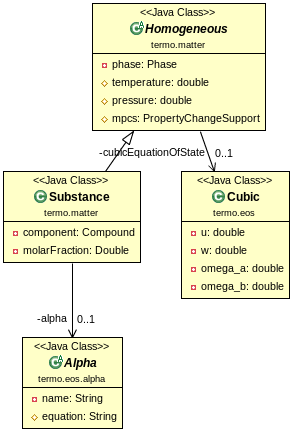
\includegraphics[scale=0.7]{cubic.png}
    \caption{A picture of a gull.}
\end{figure}


%hecho

		\subsection{Entalpía}

\begin{equation}
h = h^{\neq} + \left[ \frac{T(\frac{\partial a}{\partial T}) - a}{b\sqrt{u²-4w} }\right] 
\ln\left[\frac{2v+b\left(u + \sqrt{u²-4w}\right)}{2v+b\left(u - \sqrt{u²-4w}\right)}\right]
+ pv - RT
\end{equation}

\begin{lstlisting}[label=some-code,caption=Some Code]
private  double calculateEnthalpy( double volume){
    double idealGasEnthalpy = calculateIdealGasEnthalpy();
    double a = calculate_a_cubicParameter();
    double b = calculate_b_cubicParameter();
    double L = cubicEquationOfState.calculateL(volume, b);
    double partial_aPartial_temperature = partial_aPartial_temperature( );
    
    return idealGasEnthalpy + ((partial_aPartial_temperature - a)/b) * L  + pressure * volume - Constants.R *temperature;
}
\end{lstlisting}	


\subsubsection{Entalpía del gas ideal}
\begin{equation}
h^{\neq} = \sum_{i=1}^{nc} x_i \left[ h_i^{ref} + \int_{Tref}^{T} Cp_i^{\neq} \mathrm{d}T \right]
\end{equation}



\begin{tikzpicture}
\begin{axis}
\addplot[blue]table{plotdata/enthalpy/lv.dat};
\end{axis}
\end{tikzpicture}


%\addplot+[point meta=explicit]table[x=xcolname,y=ycolname,meta=colordata]{datafile.dat};%ejemplo de uso meta
\begin{tikzpicture}
\begin{axis}[view/h=-165]
\addplot3[surf,point meta=explicit]table[meta=temperature]{plotdata/enthalpy/lv3d.dat};
\addplot3[surf,point meta=explicit]table[meta=temperature]{plotdata/enthalpy/l3d.dat};
\addplot3[surf,point meta=explicit]table[meta=temperature]{plotdata/enthalpy/v3d.dat};
\end{axis}
\end{tikzpicture}
\begin{tikzpicture}
\begin{axis}[view/h=-225]
\addplot3[surf]table{plotdata/enthalpy/lv3d.dat};
\addplot3[surf]table{plotdata/enthalpy/l3d.dat};
\addplot3[surf]table{plotdata/enthalpy/v3d.dat};
\end{axis}
\end{tikzpicture}
\begin{tikzpicture}
\begin{axis}[view/h=-120]
\addplot3[surf]table{plotdata/enthalpy/lv3d.dat};
\addplot3[surf]table{plotdata/enthalpy/l3d.dat};
\addplot3[surf]table{plotdata/enthalpy/v3d.dat};
\end{axis}
\end{tikzpicture}	

		
		\subsection{Expresiones de $\alpha$}

	\subsubsection{Soave\cite{soave}}

\begin{gather}
	\alpha^{\nicefrac{1}{2}} = 1 + m \left(1-\sqrt{T_r}\right)\\
	m = 0.48508+1.55171\omega-0.15613\omega^2
\end{gather}
	\subsubsection{Peng and Robinson \cite{pengRobinson}}


\begin{gather}
	\alpha^{\nicefrac{1}{2}} = 1 + m \left(1-\sqrt{T_r}\right)\\
	m = 0.37464+1.54226\omega-0.2699\omega^2
\end{gather}
	\subsubsection{Mathias\cite{mathias} }
\begin{itemize}

\item{$T < T_C$}
\begin{gather}
	\alpha^{\nicefrac{1}{2}} = 1 + m \left(1-\sqrt{T_r}\right)- A\left(1-T_r\right)\left(0.7-T_r\right)
	\\
	m = 0.48508+1.55191\omega-0.15613\omega^2
\end{gather}

\item{$T > T_c$}
\begin{gather}
	\alpha = \exp{\left[ \left( \frac{c-1}{c} \right)  \left(  1- T_r^c  \right)  \right]}\\
	c = 1 + \frac{m}{2} + 0.3 A
\end{gather}

 \end{itemize}


	\subsubsection{Stryjek and Vera(PRSV)\cite{stryjekVeraPureCompounds} }
\begin{itemize}

\item{$T < T_C$}
\begin{gather}
	\alpha^{\nicefrac{1}{2}} = 1 + \kappa_0 \left(1-\sqrt{T_r}\right)- \kappa_1\left(1-T_r\right)\left(0.7-T_r\right)
	\\
	\kappa_0 = 0.378893+1.4897153\omega-0.17131848\omega^2+0.0196554\omega³
\end{gather}

\item{$T > T_c$}
\begin{equation}
	\alpha^{\nicefrac{1}{2}} = 1 + \kappa_0\left(1- \sqrt{T_r}\right)
\end{equation}

 \end{itemize}	
	\subsubsection{Adachi and Lu \cite{adachiLu}}

\begin{equation}
\alpha = A\cdot {10}^{B\left(1-T_r\right)}
\end{equation}
	\subsubsection{Soave \cite{soaveR}}

\begin{equation}
\alpha= 1+\left(1-T_r\right)\left(A + \frac{B}{T_r}\right)
\end{equation}
	\subsubsection{Melhem, et al.\cite{melhem}}

\begin{equation}
\ln{\alpha}=A\left(1-T_r\right)+ B\left(1-\sqrt{T_r}\right)^2
\end{equation}
	\subsubsection{Androulakis,et al.\cite{androulakis}}

\begin{itemize}
\item{$T < T_C$}
\begin{equation}
 \alpha = 1 + A \left(1-T_r^{\nicefrac{2}{3}}\right) + B\left(1-T_r^{\nicefrac{2}{3}}\right)^2+ C\left(1-T_r^{\nicefrac{2}{3}}\right)^3
\end{equation}
\item{$T > T_c$}
\begin{equation}
\alpha = \mathrm{e}^{A\left(1-T_r^{\nicefrac{2}{3}}\right)}
\end{equation}
\end{itemize}
	\subsubsection{Mathias and Copeman. \cite{mathiasCopeman,michelsen}}

\begin{itemize}
\item{$T < T_c$}
\begin{equation}
\alpha^{\nicefrac{1}{2}} = 1 + A\left(1-\sqrt{T_r}\right) + B\left(1-\sqrt{T_r}\right)^2 + C\left(1-\sqrt{T_r}\right)^3
\end{equation}
\item{$T > T_c$}
\begin{equation}
\alpha^{\nicefrac{1}{2}} = 1 + A\left(1-\sqrt{T_r}\right)\footnote{La ecuación no se incluyó en el trabajo original de Mathias and Copeman\cite{mathiasCopeman}; esta expresión fue incorporada en el trabajo de Dahl and Michelsen \cite{michelsen}}
\end{equation}
\end{itemize}
	\subsubsection{Yu and Lu\cite{yuLu}}

\begin{itemize}
\item{$T < T_c$}
\begin{equation}
 \log_{10}{\alpha} = \left(A+B T_r+ C T_r^2\right)\left(1-T_r\right)
\end{equation}
\item{$T > T_c$}
\begin{equation}
 \log_{10}{\alpha} = \left(A+B+C \right)\left(1-T_r\right)
\end{equation}
\end{itemize}
	\subsubsection{Stryjek and Vera\cite{stryjekVera}}

\begin{itemize}
\item{$T < T_c$}
\begin{gather}
\alpha^{\nicefrac{1}{2}} = 1 + \kappa\left(1-\sqrt{T_r}\right)\\
\kappa = m + \left[
		A+ B\left(C- T_r\right)\left(1-\sqrt{T_r}\right)
	\right]
	\left[
		\left(1+ \sqrt{T_r}\right)\left(0.7-T_r\right)
	\right]\\
m=0.378893 + 1.4897153 \omega - 0.17131848 \omega^2+ 0.0196554 \omega^3
\end{gather}
\item{$T > T_c$}
\begin{equation}
\alpha^{\nicefrac{1}{2}} = 1 + m\left(1-\sqrt{T_r}\right)
\end{equation}
\end{itemize}
	\subsubsection{Twu\cite{twuequation}}
\begin{equation}
	\alpha = T_r^{N\left(M-1\right)}\exp{\left(L\left(1-T_r^{N M}\right)\right)}
\end{equation}
	\subsubsection{Twu \cite{twuactivity}}
\begin{itemize}
\item{$T < T_c$}
\begin{gather}
\alpha = \alpha^{(0)} + \omega\left(\alpha^{(1)}-\alpha^{(0)}\right)\\
\text{Para}\qquad \alpha^{(0)}\notag\\
L= 0.196545\qquad M=0.906437\qquad N=1.26251\\
\text{Para}\qquad \alpha^{(1)}\notag\\
L=0.704001 \qquad M =0.790407 \qquad N=2.13076
\end{gather}
\item{$T > T_c$}
\begin{gather}
\alpha = \alpha^{(0)} + \omega\left(\alpha^{(1)}-\alpha^{(0)}\right)\\
\text{Para}\qquad \alpha^{(0)}\notag\\
L= 0.358826\qquad M=4.23478\qquad N=-0.2\\
\text{Para}\qquad \alpha^{(1)}\notag\\
L=0.0206444 \qquad M =1.22942 \qquad N=-8.0
\end{gather}
\end{itemize}
	\subsubsection{GCEOS (AspenHYSYS)}

\begin{gather}
\alpha^{\nicefrac{1}{2}} = 1 + \kappa \left(1 - \sqrt{T_r}\right)\\
\kappa = \kappa_0 + \left[ 
	\kappa_1 + \left(   \kappa_2 - \kappa_3 T_r   \right)
	\left(1 - T_r^{\kappa_4}\right) 
\right]
\left[
	\left(1 + \sqrt{T_r}\right)\left(0.7 - T_r\right)
\right]
T^{\kappa_5}\\
\kappa_0 = A + B \omega+ C \omega^2+ D \omega^3
\end{gather}









		
		\subsection{Fugacidad}

\begin{multline}
\ln\hat{\phi_i} = - \ln\left(\frac{v-b}{v}\right) 
+ (z-1)\left[\frac{1}{b}\frac{\partial bN}{\partial N_i}\right]
+ \frac{a}{RTb\sqrt{u^2-4w}}
\\
\left[\frac{1}{b}\frac{\partial bN}{\partial N_i}
- \frac{1}{aN}\frac{\partial aN²}{\partial N_i}\right]
\ln\left[\frac{2v+b\left(u + \sqrt{u²-4w}\right)}{2v+b\left(u - \sqrt{u²-4w}\right)}\right]
-\ln{z}
\end{multline}
		
		\subsection{Entropía}
\begin{equation}
s = s^{\neq} + R\ln\left[\frac{z(v-b)}{v}\right] + \frac{\frac{\partial a}{\partial T}}{b \sqrt{u^2 - 4w}}
\ln\left[\frac{2v+b\left(u + \sqrt{u²-4w}\right)}{2v+b\left(u - \sqrt{u²-4w}\right)}\right]
\end{equation}
\begin{equation}
s^{\neq} = \sum_{i=1}^{nc} x_i\left[s_i^{ref} + \int_{Tref}^T \frac{Cp_i^{\neq}}{T} \mathrm{d}T 
- R\ln \left(\frac{p}{p_{ref}}\right)- R\ln{x_i}
\right]
\end{equation}
		\subsection{Energía libre de Gibbs}

\begin{equation}
g = h - T * s;
\end{equation}
		
		\subsection{volumen molar}
		\subsection{Equilibrio LV}
			\subsubsection{Temperatura de Burbuja}



\begin{tikzpicture}[nodes={draw, fill=white,align=center},row sep=0.3cm,column sep=0.5cm] ]

\node(init){Inicio};
\node[below of=init] (lab)  {Lectura de \textbf{Datos} \\$P,x_1, x_2,\ldots, x_{nc}$};
\node[below of=lab,below](estim){Estimado inicial de\\ las incognitas\\$T,y_1,y_2,\ldots,y_{nc}$};
\node[below of=estim,below](relations){Cálculo de las\\ razones de equilibrio\\
$K_i = \frac{ \hat{\phi}_i^L }{\hat{ \phi}_i^V}$};
\node[below of=relations,below = 0.2cm](error){Cálculo de la función Error\\$ S_y =\sum_{i=1}^{nc} K_i x_i $\\$ E = \ln{S_y} $};

\node[below of=error,below](criteria){$|E| \leq 1\cdot10^{-4}\quad \text{o} \quad  1\cdot 10^{-5}$};
\node[below of=criteria,below](tempIncrement){Incrementer la temperatura\\$T^* = T + \Delta T$\\
$\Delta T = 0.1  \quad \text{o} \quad 1.0 K$};

\node[below of=tempIncrement,below](relationsWithIncrement){Cálculo de las Razones\\ de Equilibrio con $T^*$
\\$K_i^* = \frac{ \hat{\phi}_i^L }{ \hat{\phi}_i^V}$};

\node[right of=criteria	,right=2.2cm](end){Fin};


\node[right of=tempIncrement, right=3cm](errorWithIncrement){Cálculo de la función Error \\ con $T^*$\\
$ S_y^* =\sum_{i=1}^{nc} K_i^* x_i $\\$ E^* = \ln{S_y^*} $};

\node[right of=relations, right = 3cm](newValues){Cálculo de las nuevas estimaciones \\ de las \textbf{Incógnitas}\\
\begin{minipage}{0.2\linewidth}
\begin{equation*}
T_{nueva} = \frac{TT^* \left(E^*-E\right)}{T^*E^*-TE}
\end{equation*}
\begin{equation*}
 S_y =\sum_{i=1}^{nc} K_i x_i \\
 \end{equation*}
 \begin{equation*}
\left(y_i\right)_{nueva} = \frac{K_i x_i}{S_y}
\end{equation*}
\end{minipage}
};


\draw[-latex] (init)--(lab);
\draw[-latex] (lab)--(estim);
\draw[-latex] (estim)--(relations);
\draw[-latex] (relations)--(error);
\draw[-latex] (error)--(criteria);
\draw[-latex] (criteria)--node[fill=none,draw=none,above]{SI}(end);
\draw[-latex] (criteria)--node[fill=none,draw=none,left]{NO}(tempIncrement);
\draw[-latex] (tempIncrement)--(relationsWithIncrement);
\draw[-latex] (relationsWithIncrement)--(errorWithIncrement);
\draw[-latex] (errorWithIncrement)--(newValues);
\draw[-latex] (newValues)--(relations);

\end{tikzpicture}

		\subsubsection{Temperatura de Rocío}



\begin{tikzpicture}[nodes={draw, fill=white,align=center},row sep=0.3cm,column sep=0.5cm] ]

\node(init){Inicio};
\node[below of=init] (lab)  {Lectura de \textbf{Datos} \\$P,y_1, y_2,\ldots, y_{nc}$};
\node[below of=lab,below](estim){Estimado inicial de\\ las incognitas\\$T,x_1,x_2,\ldots,x_{nc}$};
\node[below of=estim,below](relations){Cálculo de las\\ razones de equilibrio\\
$K_i = \frac{ \hat{\phi}_i^L }{ \hat{ \phi}_i^V}$};
\node[below of=relations,below = 0.2cm](error){Cálculo de la función Error\\
$ S_x =\sum_{i=1}^{nc}\frac{y_i}{ K_i} $\\$ E = \ln{S_x} $};

\node[below of=error,below](criteria){$|E| \leq 1\cdot10^{-4}\quad \text{o} \quad  1\cdot 10^{-5}$};
\node[below of=criteria,below](tempIncrement){Incrementer la temperatura\\$T^* = T + \Delta T$\\
$\Delta T = 0.1  \quad \text{o} \quad 1.0 K$};

\node[below of=tempIncrement,below](relationsWithIncrement){Cálculo de las Razones\\ de Equilibrio con $T^*$\\$K_i^* = \frac{ \hat{\phi}_i^L }{\hat{\phi}_i^V}$};

\node[right of=criteria	,right=2.2cm](end){Fin};


\node[right of=tempIncrement, right=3cm](errorWithIncrement){Cálculo de la función Error \\ con $T^*$\\
$ S_x^* =\sum_{i=1}^{nc} \frac{y_i}{K_i^*}  $\\$ E^* = \ln{S_x^*} $};

\node[right of=relations, right = 3cm](newValues){Cálculo de las nuevas estimaciones \\ de las \textbf{Incógnitas}\\
\begin{minipage}{0.2\linewidth}
\begin{equation*}
T_{nueva} = \frac{TT^* \left(E^*-E\right)}{T^*E^*-TE}
\end{equation*}
\begin{equation*}
 S_x =\sum_{i=1}^{nc}\frac{y_i}{K_i}   \\
 \end{equation*}
 \begin{equation*}
\left(x_i\right)_{nueva} = \frac{y_i}{K_i S_x}
\end{equation*}
\end{minipage}
};


\draw[-latex] (init)--(lab);
\draw[-latex] (lab)--(estim);
\draw[-latex] (estim)--(relations);
\draw[-latex] (relations)--(error);
\draw[-latex] (error)--(criteria);
\draw[-latex] (criteria)--node[fill=none,draw=none,above]{SI}(end);
\draw[-latex] (criteria)--node[fill=none,draw=none,left]{NO}(tempIncrement);
\draw[-latex] (tempIncrement)--(relationsWithIncrement);
\draw[-latex] (relationsWithIncrement)--(errorWithIncrement);
\draw[-latex] (errorWithIncrement)--(newValues);
\draw[-latex] (newValues)--(relations);

\end{tikzpicture}

		\subsubsection{Presión de Burbuja}




\begin{tikzpicture}[nodes={draw, fill=white,align=center},row sep=0.3cm,column sep=0.5cm] ]

\node(init){Inicio};
\node[below of=init] (lab)  {Lectura de \textbf{Datos} \\$T,x_1, x_2,\ldots, x_{nc}$};
\node[below of=lab,below](estim){Estimado inicial de\\ las incognitas\\$P,y_1,y_2,\ldots,y_{nc}$};
\node[below of=estim,below](relations){Cálculo de las\\ razones de equilibrio\\
$K_i = \frac{ \hat{\phi}_i^L }{\hat{ \phi}_i^V}$};
\node[below of=relations,below = 0.2cm](error){Cálculo de la función Error\\$ S_y =\sum_{i=1}^{nc} K_i x_i $\\$ E = {S_y}-1 $};

\node[below of=error,below](criteria){$|E| \leq 1\cdot10^{-4}\quad \text{o} \quad  1\cdot 10^{-5}$};
\node[below of=criteria,below](pressureIncrement){Incrementer la temperatura\\$P^* = P + \Delta P$\\
$\Delta P = 0.001  \quad \text{o} \quad 0.0001 K$};

\node[below of=pressureIncrement,below](relationsWithIncrement){Cálculo de las Razones\\ de Equilibrio con $P^*$
\\$K_i^* = \frac{ \hat{\phi}_i^L }{ \hat{\phi}_i^V}$};

\node[right of=criteria	,right=2.2cm](end){Fin};


\node[right of=pressureIncrement, right=3cm](errorWithIncrement){Cálculo de la función Error \\ con $P^*$\\
$ S_y^* =\sum_{i=1}^{nc} K_i^* x_i $\\$ E^* = S_y^* -1 $};

\node[right of=relations, right = 3cm](newValues){Cálculo de las nuevas estimaciones \\ de las \textbf{Incógnitas}\\
\begin{minipage}{0.2\linewidth}
\begin{equation*}
T_{nueva} = \frac{P P^* \left(E^*-E\right)}{P^*E^*-P E}
\end{equation*}
\begin{equation*}
 S_y =\sum_{i=1}^{nc} K_i x_i \\
 \end{equation*}
 \begin{equation*}
\left(y_i\right)_{nueva} = \frac{K_i x_i}{S_y}
\end{equation*}
\end{minipage}
};


\draw[-latex] (init)--(lab);
\draw[-latex] (lab)--(estim);
\draw[-latex] (estim)--(relations);
\draw[-latex] (relations)--(error);
\draw[-latex] (error)--(criteria);
\draw[-latex] (criteria)--node[fill=none,draw=none,above]{SI}(end);
\draw[-latex] (criteria)--node[fill=none,draw=none,left]{NO}(pressureIncrement);
\draw[-latex] (pressureIncrement)--(relationsWithIncrement);
\draw[-latex] (relationsWithIncrement)--(errorWithIncrement);
\draw[-latex] (errorWithIncrement)--(newValues);
\draw[-latex] (newValues)--(relations);

\end{tikzpicture}

		\subsubsection{Presión de Rocío}



\begin{tikzpicture}[nodes={draw, fill=white,align=center},row sep=0.3cm,column sep=0.5cm] ]

\node(init){Inicio};
\node[below of=init] (lab)  {Lectura de \textbf{Datos} \\$T,y_1, y_2,\ldots, y_{nc}$};
\node[below of=lab,below](estim){Estimado inicial de\\ las incognitas\\$P,x_1,x_2,\ldots,x_{nc}$};
\node[below of=estim,below](relations){Cálculo de las\\ razones de equilibrio\\
$K_i = \frac{ \hat{\phi}_i^L }{ \hat{ \phi}_i^V}$};
\node[below of=relations,below = 0.2cm](error){Cálculo de la función Error\\
$ S_x =\sum_{i=1}^{nc}\frac{y_i}{ K_i} $\\$ E = S_x-1 $};

\node[below of=error,below](criteria){$|E| \leq 1\cdot10^{-4}\quad \text{o} \quad  1\cdot 10^{-5}$};
\node[below of=criteria,below](tempIncrement){Incrementer la temperatura\\$P^* = P + \Delta P$\\
$\Delta P = 0.001  \quad \text{o} \quad 0.0001 K$};

\node[below of=tempIncrement,below](relationsWithIncrement){Cálculo de las Razones\\ de Equilibrio con $P^*$\\$K_i^* = \frac{ \hat{\phi}_i^L }{\hat{\phi}_i^V}$};

\node[right of=criteria	,right=2.2cm](end){Fin};


\node[right of=tempIncrement, right=3cm](errorWithIncrement){Cálculo de la función Error \\ con $P^*$\\
$ S_x^* =\sum_{i=1}^{nc} \frac{y_i}{K_i^*}  $\\$ E^* = S_x^*-1 $};

\node[right of=relations, right = 3cm](newValues){Cálculo de las nuevas estimaciones \\ de las \textbf{Incógnitas}\\
\begin{minipage}{0.2\linewidth}
\begin{equation*}
T_{nueva} =P- \frac{E  \left(P^*-P\right)}{E^*-E}
\end{equation*}
\begin{equation*}
 S_x =\sum_{i=1}^{nc}\frac{y_i}{K_i}   \\
 \end{equation*}
 \begin{equation*}
\left(x_i\right)_{nueva} = \frac{y_i}{K_i S_x}
\end{equation*}
\end{minipage}
};


\draw[-latex] (init)--(lab);
\draw[-latex] (lab)--(estim);
\draw[-latex] (estim)--(relations);
\draw[-latex] (relations)--(error);
\draw[-latex] (error)--(criteria);
\draw[-latex] (criteria)--node[fill=none,draw=none,above]{SI}(end);
\draw[-latex] (criteria)--node[fill=none,draw=none,left]{NO}(tempIncrement);
\draw[-latex] (tempIncrement)--(relationsWithIncrement);
\draw[-latex] (relationsWithIncrement)--(errorWithIncrement);
\draw[-latex] (errorWithIncrement)--(newValues);
\draw[-latex] (newValues)--(relations);

\end{tikzpicture}

		\subsection{Flash}



\begin{tikzpicture}[nodes={draw, fill=white,align=center},row sep=0.3cm,column sep=0.5cm] ]

\node(init){Inicio};
\node[below of=init] (lab)  {Lectura de \textbf{Datos} \\$T,P,z_1, z_2,\ldots, z_{nc}$};
\node[below of=lab,below](estim){Estimado inicial de\\ las incognitas\\$V/F,x_1,x_2,\ldots,x_{nc}$\\$y_1,y_2 \ldots, y_{nc}$};
\node[below of=estim,below](relations){Cálculo de las\\ razones de equilibrio\\
$K_i = \frac{ \hat{\phi}_i^L }{ \hat{ \phi}_i^V}$};
\node[below of=relations,below = 0.2cm](error){Cálculo de la función Error\\
$ \zeta =\sum_{i=1}^{nc}\left| x_i \hat{\varphi}_i^L - y_i \hat{\varphi}_i^V \right|$};

\node[below of=error,below](criteria){$|\zeta| \leq 1\cdot10^{-4}\quad \text{o} \quad  1\cdot 10^{-5}$};


\node[below of=criteria,below](rachford){Cálculo de $V/F$ con Rachford-Rice:\\ 
\begin{minipage}{0.5\linewidth}
\begin{equation*}
S = \sum_{i=1}^{nc}\frac{z_i\left(K_i - 1\right)}{1+ \frac{V}{F}\left(K_i-1\right)}
\end{equation*}
Encontrar $V/F$ tal que $S = 0$\\
Método de Newton-Raphson\\
\begin{equation*}
\acute{S} = \sum_{i=1}^{nc} \frac{-z_i \left(K_i - 1\right)^2}{\left[1+ \frac{V}{F} \left(K_i-1\right)\right]^2}
\end{equation*}
\begin{equation*}
\left(\frac{V}{F}\right)_{nueva} = \left(\frac{V}{F}\right) - \frac{S}{\acute{S}}
\end{equation*}
\end{minipage}};

\node[right of=criteria	,right=2.2cm](end){Fin};


\node[right of=estim, right = 3cm](newValues){Cálculo de las nuevas estimaciones \\ de las \textbf{Incógnitas}\\
\begin{minipage}{0.3\linewidth}
\begin{equation*}
\acute{x_i} = \frac{z_i}{1 + \frac{V}{F}\left(K_i-1\right)}
\end{equation*}
\begin{equation*}
 S_x =\sum_{i=1}^{nc}\acute{x}_i \qquad x_i = \frac{\acute{x_i}}{S_x}
\end{equation*}
\begin{equation*}
\acute{y_i} = \acute{x_i} K_i = \frac{z_i K_i}{1+\frac{V}{F}\left(K_i - 1\right)}
\end{equation*}
\begin{equation*}
 S_y =\sum_{i=1}^{nc}\acute{y}_i \qquad y_i = \frac{\acute{y_i}}{S_y}
\end{equation*}
\end{minipage}
};


\draw[-latex] (init)--(lab);
\draw[-latex] (lab)--(estim);
\draw[-latex] (estim)--(relations);
\draw[-latex] (relations)--(error);
\draw[-latex] (error)--(criteria);
\draw[-latex] (criteria)--node[fill=none,draw=none,above]{SI}(end);
\draw[-latex] (criteria)--node[fill=none,draw=none,left]{NO}(rachford);

\draw[-latex] (rachford)-|(newValues);
\draw[-latex] (newValues)--(relations);

\end{tikzpicture}

		\subsection{Diagramas}
	



	\chapter{Optimización de parámetros}
	\section{Parámetros de $\alpha$}

	\section{Parámetros binarios}

\begin{tikzpicture}
\begin{axis}
\addplot[blue,only marks]table[x=temperature, y=exppressure]{plotdata/alphaOptimization/error.dat};
\addplot[red]table[x=temperature,y=calcpressure]{plotdata/alphaOptimization/error.dat};
\end{axis}
\end{tikzpicture}



\begin{tabular}{c c c}
\begin{tikzpicture}
	\begin{axis}
		\addplot[red,only marks]table[x=temperature,y=error]{plotdata/alphaOptimization/error.dat};
		\addplot[blue,only marks]table[x=temperature,y=error]{plotdata/alphaOptimization/minError.dat};
	\end{axis}
\end{tikzpicture}
&
\begin{tikzpicture}
	\begin{axis}[width=5cm]
	\addplot[blue,only marks]table[x=temperature,y=error]{plotdata/alphaOptimization/minError.dat};
	\end{axis}
\end{tikzpicture}
\end{tabular}





\begin{tikzpicture}
\begin{axis}
\addplot[yellow,only marks]table[x=iteration,y=a]{plotdata/alphaOptimization/trayectory2dimension.dat};
\addplot[green,only marks]table[x=iteration,y=b]{plotdata/alphaOptimization/trayectory2dimension.dat};
\end{axis}
\begin{axis}

\addplot[blue,only marks]table[x=iteration,y=error]{plotdata/alphaOptimization/trayectory2dimension.dat};
\end{axis}
\end{tikzpicture}


\begin{tikzpicture}
\begin{axis}% [view/v=45]
\addplot3[surf]table{plotdata/alphaOptimization/params.dat};
\addplot3[red]table{plotdata/alphaOptimization/trayectory.dat};
\end{axis}
\end{tikzpicture}
	\chapter{Optimización de parámetros $Binarios$}


\definecolor{amber}{rgb}{1.0, 0.49, 0.0}

\newcommand{\binaryDiagram}[1] {
\begin{tikzpicture}
\begin{axis}
\addplot[amber,only marks,mark size = 1pt]table[x=x1, y=expTemp]{#1};
\addplot[blue,only marks,mark size = 1pt]table[x=yExp, y=expTemp]{#1};
\addplot[green,thick] table[x=x1, y=calcTemp]{#1};
\addplot[red,thick] table[x=yCalc, y=calcTemp]{#1};
\end{axis}
\end{tikzpicture}
 }

\binaryDiagram{plotdata/binaryOptim/error.dat}

\binaryDiagram{plotdata/binaryOptim/errorAfterOptim.dat}
	\chapter{Paquetes termodinámicos}
	\section{Estructura de la librería}
	 \subsection{Materia Homogénea}

			\begin{figure}[!h]
			  
			  \centering
			    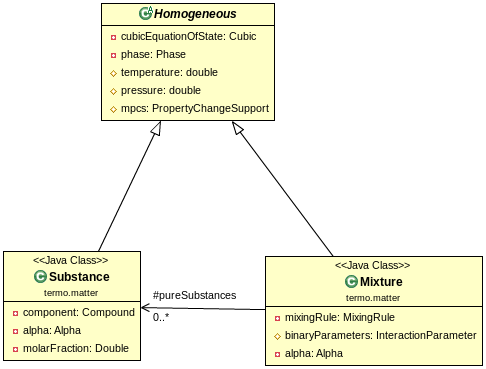
\includegraphics[scale=0.7]{Homogenous.png}
			    \caption{A picture of a gull.}
			\end{figure}

		\subsection{Materia Heterogénea}

			\begin{figure}[!h]
			  
			  \centering
			    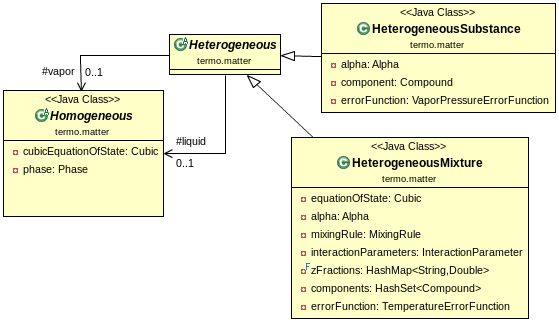
\includegraphics[scale=0.7]{heterogeneous.png}
			    \caption{ads}
			\end{figure}


	
		\subsection{Mezcla}



	\section{Objetos incluidos}
		\subsection{Ecuaciones de estado cúbicas}
		\subsection{Expresiones de $\alpha$}
		\subsection{Reglas de mezclado}
		\subsection{modelos de actividad}
	\section{¿Cómo extender los paquetes?/ ¿Cómo escribir mi propio paquete?}
		\subsection{Fork Repo desde GitHub}
		\subsection{Agregar classes}
		\subsection{Pull Request}

	\chapter{Aplicación de internet}
	\section{Base de datos}
		\subsection{Usuarios}
		\subsection{Componentes}
		\subsection{Listas de datos experimentales}
			\subsubsection{Compuestos}
			\subsubsection{Mezclas}
	
	\include{advancedOptions_chapter}
	\chapter{Diagramas ternarios}

\newcommand{\alphaOptim}[1] {

\begin{tabular}{c c}

\begin{tikzpicture}
	\begin{axis}
		\addplot[blue,only marks,mark size = 1pt]table[x=Temperature,y=experimentalPressure]{plotdata/ternaryDiagram/#1/afterOptim.dat};
		\addplot[red,thick]table[x=Temperature,y=calculatedPressure]{plotdata/ternaryDiagram/#1/afterOptim.dat};
	\end{axis}
\end{tikzpicture}
&
\begin{tikzpicture}
	\begin{axis}
		\addplot[blue,only marks,mark size = 1pt]table[x=Temperature,y=experimentalPressure]{plotdata/ternaryDiagram/#1/beforeOptim.dat};
		\addplot[red,thick]table[x=Temperature,y=calculatedPressure]{plotdata/ternaryDiagram/#1/beforeOptim.dat};
	\end{axis}
\end{tikzpicture}
\\
\begin{tikzpicture}
	\begin{axis}
		\addplot[blue,only marks,mark size = 1pt]table[x=Temperature,y=error]{plotdata/ternaryDiagram/#1/beforeOptim.dat};
		\addplot[red,only marks,mark size = 1pt]table[x=Temperature,y=error]{plotdata/ternaryDiagram/#1/afterOptim.dat};
	\end{axis}
\end{tikzpicture}
&
\begin{tikzpicture}
	\begin{axis}
		\addplot[only marks,mark size = 1pt]table[x=iteration,y=A]{plotdata/ternaryDiagram/#1/history.dat};
		\addplot[only marks,mark size = 1pt]table[x=iteration,y=B]{plotdata/ternaryDiagram/#1/history.dat};
		\addplot[only marks,mark size = 1pt]table[x=iteration,y=C]{plotdata/ternaryDiagram/#1/history.dat};
	
	\end{axis}
\end{tikzpicture}
\\
\begin{tikzpicture}
	\begin{axis}
		\addplot[red,only marks,mark size = 1pt]table[x=iteration,y=Error]{plotdata/ternaryDiagram/#1/history.dat};
	\end{axis}
\end{tikzpicture}
\end{tabular}
}


\newcommand{\binary}[1]{
\begin{tikzpicture}
	\begin{axis}
		\addplot[blue,only marks,mark size = 1pt]table[x=x1,y=pressure]{plotdata/ternaryDiagram/#1/beforeOptim.dat};
		\addplot[red,only marks,mark size = 1pt]table[x=y1,y=pressure]{plotdata/ternaryDiagram/#1/beforeOptim.dat};
		\addplot[green,thick]table[x=y1calc,y=calcpressure]{plotdata/ternaryDiagram/#1/beforeOptim.dat};
		\addplot[brown,thick]table[x=x1,y=calcpressure]{plotdata/ternaryDiagram/#1/beforeOptim.dat};

		\addplot[purple,thick]table[x=y1calc,y=calcpressure]{plotdata/ternaryDiagram/#1/afterOptim.dat};
		\addplot[black,thick]table[x=x1,y=calcpressure]{plotdata/ternaryDiagram/#1/afterOptim.dat};
	\end{axis}
\end{tikzpicture}

}

\alphaOptim{ethylene}
\alphaOptim{water}
\alphaOptim{ethanol}


binary



\binary{ethylenewater}



\begin{tikzpicture}
\begin{ternaryaxis}[xlabel=Agua,
ylabel=Etileno,
zlabel=Etanol]
\addplot3[only marks,blue] table[x=x1,y=x2,z=x3]{plotdata/ternaryDiagram/graph.dat};
\addplot3[only marks,red] table[x=y1,y=y2,z=y3]{plotdata/ternaryDiagram/graph.dat};
\end{ternaryaxis}
\end{tikzpicture}
	\appendix
	\chapter{Ejemplo de uso con Netbeans} \label{}



	\section{Requisitos}

	\begin{enumerate}

	\item Necesitamos tener instalado kit de desarrollo Jdk de java que se puede descargar desde la página (http://www.oracle.com/technetwork/java/javase/downloads/).

	\item Necesitamos tener instalado el ambiente de desarrollo Netbeans que se puede descargar de la página (https://netbeans.org/downloads/).
	\end{enumerate}

	\section{Manualmente}\label{sec:manualInstall}
		Descargar el archivo .jar y agregarlo al folder /lib de la aplicación
		\begin{enumerate}
			\item Desde la página oficial de EQ PRO(ingenieria-eqpro.rhcloud.com) se puede descargar el archivo jar.

			\item Crear un nuevo proyecto desde Netbeans.

			\begin{center}
			  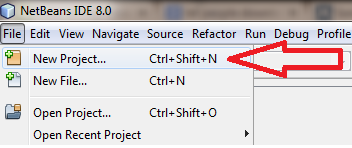
\includegraphics[scale=0.7]{new-proyect.png}
			\end{center}

			\item Elegir el tipo de aplicación java.application 
			\begin{center}
			  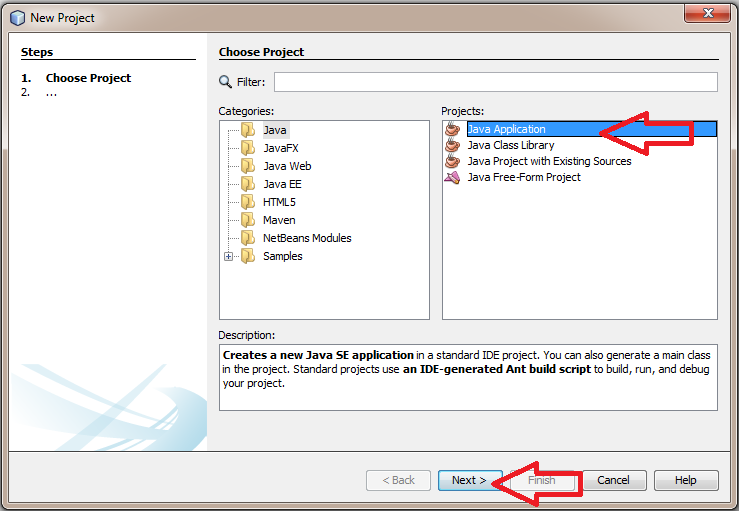
\includegraphics[scale=0.7]{application-type.png} 
			\end{center}
			\item Asignar el nombre del proyecto 
			\begin{center}
			  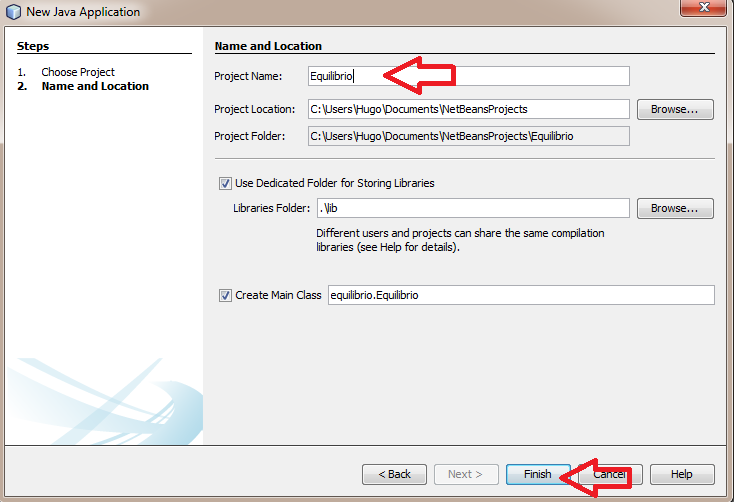
\includegraphics[scale=0.7]{proyect-name.png} 
			\end{center}
			\item En la pestaña proyectos de netbeans, con click derecho en la carpeta “Libraries” elegir la opción “Agregar jar/Folder “.
			\begin{center}
			  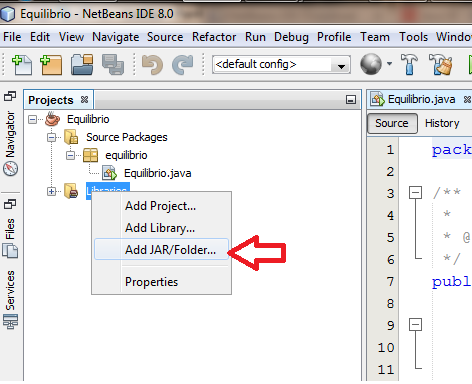
\includegraphics[scale=0.7]{add-jar.png} 
			\end{center}


			 \item Navegar entonces hasta la ruta donde se descargo el archivo jar. 

			\begin{center}
			  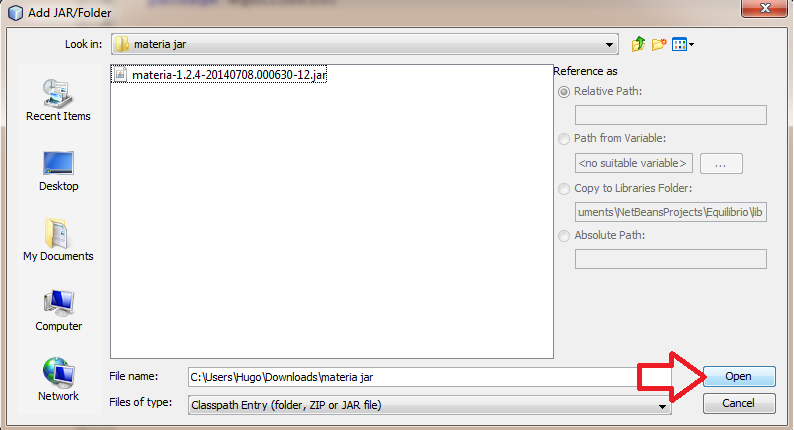
\includegraphics[scale=0.7]{select-materia-jar.png} 
			\end{center}

			Se puede ver entonces la librería agregada al proyecto.

			\begin{center}
			  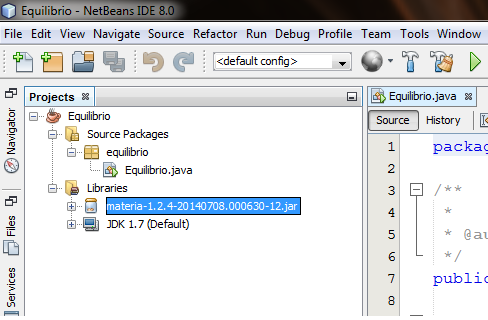
\includegraphics[scale=0.7]{library-added.png} 
			\end{center}
		\end{enumerate}

	\section{Maven}

		Desde maven utilizando el archivo pom.xml.
		    Crear nuevo proyecto :new proyect
		     Elegir la categoría ->Maven ->Java Applicationmaven java app
		    Elegir nombre del proyecto y dar click en finalizar.maven name
		    Podemos ver en la carpeta del proyecto la siguiente estructura
		\begin{verbatim}
		    Maven_Equilibrio
		    |-- pom.xml
		    `-- src
		        -- main
		           `-- java
		               `-- hugo
		                   `-- ejemplos
		                       `-- maven_equilibrio
		\end{verbatim}
		Abrimos el archivo pom.xml y agregamos las siguientes etiquetas


		\begin{lstlisting}[language=XML,morekeywords={repositories,
    repository,id,name,url,groupId,artifactId,dependencies,dependency}]
<dependencies>
  <dependency>
   <groupId>com.github.hugoredon</groupId>
   <artifactId>materia</artifactId>
   <version>1</version>
  </dependency>
</dependencies>
\end{lstlisting}


		5- Inmediatamente se ve agregada la dependencia Materia, cuando el proyecto se compile, se descargará el archivo jar automáticamente.

		maven materia added

		6.  Crear una clase java en cualquier paquete dentro de Source packages.maven create java class

		Escribimos dentro de esta clase el mismo código que en la entrada anterior.

	\section{Código}
		\begin{lstlisting}
			
		public class Equilibrio {
		 public static void main(String[] args) {
		 Compound agua = new Compound("agua");
		 agua.setCriticalTemperature(647.3);
		 agua.setCriticalPressure(2.212E7);
		 agua.setAcentricFactor(0.344861);
		 
		 Cubic cubicEquationOfState = EquationOfStateFactory.pengRobinsonBase();
		 Alpha alphaExpression = AlphaFactory.getStryjekAndVeraExpression();
		 
		 HeterogeneousSubstance substance =
		 new HeterogeneousSubstance(cubicEquationOfState, alphaExpression, agua);
		 double pressure = 101325;
		 substance.setPressure(pressure);
		 substance.bubbleTemperature();
		 double temperature = substance.getTemperature();
		 
		 System.out.println("(Presi|ó|n "+pressure+" [Pa])Temperatura de burbuja: " + temperature + "[K]");
		 }
		}

		\end{lstlisting}
		Ejecutamos el código y el resultado es:

		(Presión 101325.0 [Pa])Temperatura de burbuja: 374.5312063949659[K]
	\chapter{¿Cómo extender o modificar la librería desde el código fuente?}\label{chap:github}




\chapter{Solución de la ecuación de estado cúbica}\label{chap:cubicsolution}



\begin{equation}
z= \frac{P V}{R T}
\qquad
A=\frac{ap}{(RT)^2}
\qquad
B=\frac{bp}{RT}
\end{equation}

\begin{equation}
z^3-\left[1-(u-1)B\right]z^2+ \\ \left[A-uB-uB^2 +\\ wB^2\right]z-\left[AB+wB^2+wB^3\right]=0
\end{equation}


\begin{align}
\alpha &= 1-(u-1)B\\
\beta &= A -uB-uB^2+wB^3\\
\gamma &= AB +wB^2+ 2B^3\\
C &= 3\beta - \alpha^2\\
D&= - \alpha^3+ 4.5 \alpha \beta -13.5 \gamma\\
Q&=C^3+D^2
\end{align}


\begin{itemize}
\item Si $Q \leq 0 \qquad \vartheta = \arccos \left[\frac{-D}{\sqrt{-C^3}}\right]$
\begin{description}
\item{Líquido} $z = \frac{1}{3}\left[\alpha + 2 \sqrt{-C} \cos\left(\frac{\vartheta}{3} + 120\degree \right)\right]$
\item{Vapor} $z = \frac{1}{3}\left[\alpha + 2 \sqrt{-C} \cos\left(\frac{\vartheta}{3}\right)\right]$
\end{description}
Nota: En caso de que el z del líquido sea menor que B, entonces hay que calcularla como si fuera vapor.
\item Si $Q > 0 \qquad z = \frac{1}{3}\left[\alpha + \left(-D + \sqrt{Q}\right)^{\frac{1}{3}}+ \left(-D - \sqrt{Q}\right)^{\frac{1}{3}} \right]$
\end{itemize}
	\chapter{Ecuaciones}



\begin{equation}\label{eq:pressure}
P = \frac{R T}{v-b} - \frac{a}{v^2 +u b v + w b^2 }
\end{equation}


\begin{itemize}\itemsep0ex
\item $P$ : presión en $[Pa]$.
\item $v$ : volumen molar en $[\frac{m^3}{kg}]$
\item $a$ : Es una medida de la atracción entre las partículas. $[\frac{m^5}{kg s}]$
\item $b$ : volumen excluido por un mol de partículas.$[\frac{m^3}{kg}]$
\item $u$ y $w$ : Son los parámetros diferentes para cada ecuación de estado, ver tabla \ref{tab:cubics}
\item $R$ : Constante universal de los gases ideales en $\frac{m^3 Pa}{kgmol K}$
\end{itemize}


\begin{equation}\label{eq:a}
	b_i = \Omega_b \frac{R T_{ci}}{p_{ci}} 
\end{equation}

\begin{equation}\label{eq:b}
 a_i = \Omega_a \frac{\left(R T_{ci}\right)^2}{p_{ci}} \alpha_i
\end{equation}


\begin{equation}\label{eq:z}
z= \frac{P V}{R T}
\end{equation}

\begin{equation}\label{eq:volume}
V = \frac{R T}{z P}
\end{equation}

\begin{equation}\label{eq:AB}
A=\frac{ap}{(RT)^2}
\qquad
B=\frac{bp}{RT}
\end{equation}

\begin{equation}
z^3-\left[1-(u-1)B\right]z^2+ \\ \left[A-uB-uB^2 +\\ wB^2\right]z-\left[AB+wB^2+wB^3\right]=0
\end{equation}


\subsubsection{Entalpía del gas ideal}
\begin{equation}\label{eq:idealgasenthalpy}
h^{\neq} = \sum_{i=1}^{nc} x_i \left[ h_i^{ref} + \int_{Tref}^{T} Cp_i^{\neq} \mathrm{d}T \right]
\end{equation}

\section{Entalpía}
\begin{equation}\label{eq:enthalpy}
h = h^{\neq} + \left[ \frac{T(\frac{\partial a}{\partial T}) - a}{b\sqrt{u²-4w} }\right] 
\ln\left[\frac{2v+b\left(u + \sqrt{u²-4w}\right)}{2v+b\left(u - \sqrt{u²-4w}\right)}\right]
+ pv - RT
\end{equation}

\begin{lstlisting}[label=some-code,caption=Some Code]
private  double calculateEnthalpy( double volume){
    double idealGasEnthalpy = calculateIdealGasEnthalpy();
    double a = calculate_a_cubicParameter();
    double b = calculate_b_cubicParameter();
    double L = cubicEquationOfState.calculateL(volume, b);
    double partial_aPartial_temperature = partial_aPartial_temperature( );
    
    return idealGasEnthalpy + ((partial_aPartial_temperature - a)/b) * L  + pressure * volume - Constants.R *temperature;
}
\end{lstlisting}	



\subsection{Entropía}
\begin{equation}
s = s^{\neq} + R\ln\left[\frac{z(v-b)}{v}\right] + \frac{\frac{\partial a}{\partial T}}{b \sqrt{u^2 - 4w}}
\ln\left[\frac{2v+b\left(u + \sqrt{u²-4w}\right)}{2v+b\left(u - \sqrt{u²-4w}\right)}\right]
\end{equation}
\begin{equation}
s^{\neq} = \sum_{i=1}^{nc} x_i\left[s_i^{ref} + \int_{Tref}^T \frac{Cp_i^{\neq}}{T} \mathrm{d}T 
- R\ln \left(\frac{p}{p_{ref}}\right)- R\ln{x_i}
\right]
\end{equation}


\begin{equation}\label{eq:gibbs}
g = h - T * s;
\end{equation}


\begin{multline}\label{eq:fugacity}
\ln\hat{\phi_i} = - \ln\left(\frac{v-b}{v}\right) 
+ (z-1)\left[\frac{1}{b}\frac{\partial bN}{\partial N_i}\right]
+ \frac{a}{RTb\sqrt{u^2-4w}}
\\
\left[\frac{1}{b}\frac{\partial bN}{\partial N_i}
- \frac{1}{aN}\frac{\partial aN²}{\partial N_i}\right]
\ln\left[\frac{2v+b\left(u + \sqrt{u²-4w}\right)}{2v+b\left(u - \sqrt{u²-4w}\right)}\right]
-\ln{z}
\end{multline}
	\chapter{Herramientas para la página de internet}\label{chap:webTools}

\begin{itemize}
	\item Java Enterprise Edition
	\item Java Server Faces
	\item Hibernate
	\item MySQL
	\item Enterprise Java Beans 3
	\item Wildfly
	\item Openshift
	\item HTML, CSS
	\item Javascript JQuery
\end{itemize}


\section{Openshift}
		OpenShift es una plataforma de programación en la nube orientada a servicios de Red Hat. Una versión para la nube privada se llama OpenShift Enterprise. El software que ejecuta el servicio se encuentra bajo el nombre `OpenShift Origin' de código abierto y está disponible en GitHub.

\section{Wildfly}
	WildFly, anteriormente conocido como `JavaBeans Open Source Software Application Server' es un servidor de aplicaciones que implementa la plataforma Java Enterprise Edition. JBoss está escrito en Java y como tal es multiplataforma: utilizable en cualquier sistema operativo que soporte Java

	\bibliographystyle{babplain}
	\bibliography{bib/bibliography}  
\end{document} 